%
% $Id: SANDtemplate.tex,v 1.3 2007-12-13 21:27:14 rolf Exp $
% A template to build SAND reports. See the examples for more details and
% formatting suggestions. A command reference is available at
% http://www.cs.sandia.gov/~rolf/SANDreport
%
\documentclass[pdf,12pt,report,strict]{SANDreport}
%% ------------------------------------------------------------
%% PACKAGES
%% ------------------------------------------------------------

%% For \circledast
\usepackage{amssymb,amsfonts,amsmath}

\usepackage{algorithm}
%\usepackage{algorithmic}
\usepackage[noend]{algpseudocode}

%% For \mathscr
\usepackage[mathscr]{eucal}

%% For \llbracket and \rrbracket, \varoast, \varoslash
\usepackage{stmaryrd}

%% For \boldsymbol
\usepackage{amsbsy}

%% For \bm (bold math)
\usepackage{bm}

%% For \set, \Set
\usepackage{braket}

%% For \multirow
\usepackage{multirow}

%% For "X" columntype that automatically calculates width
%\usepackage{tabularx}
%\newcolumntype{Y}{>{\raggedright\arraybackslash}X}

%% For \sfrac
\usepackage{xfrac}

%% For attractive boxed equations
%% https://tex.stackexchange.com/questions/20575/attractive-boxed-equations
%usepackage{empheq}
%usepackage[most]{tcolorbox}

%% For special macros
\usepackage{xparse}

%% For special environments
\usepackage{environ}

%% For straight quote in verbatim 
\usepackage{upquote}

%% For boxed verbatim
\usepackage{moreverb}

%% For \FloatBarrier
\usepackage{placeins}

%% For pretty lists
\usepackage{enumitem}

%% Tikz - For making pretty pictures
\usepackage{tikz}
\usetikzlibrary{calc}
% \usetikzlibrary{3d}
% \usetikzlibrary{patterns}
% \usetikzlibrary{arrows}
% \usetikzlibrary{decorations.pathreplacing}

%% For plots
\usepackage{pgfplots}

%% Subfloats
\usepackage[font=footnotesize,justification=Centering,singlelinecheck=false]{subfig}

%% Redundant but causes emacs to do useful things
\usepackage{cleveref}

%% For trimming the PNG images by px
%\pdfpxdimen=\dimexpr 1 in/96\relax

\usepackage{setspace}

%% ------------------------------------------------------------
%% MACROS - USING XPARSE METHODS FOR DEFINITION
%% ------------------------------------------------------------

\definecolor{grey}{RGB}{100,100,100}
%KDD\algrenewcommand{\algorithmiccomment}[1]{\hfill\textcolor{grey}{// #1}}

\newenvironment{inlinemath}{$}{$}

% Quad-text-quad
\NewDocumentCommand \qtext {m} {\quad\text{#1}\quad}

% Reals
\NewDocumentCommand \Real {} {\mathbb{R}}

% Natural numbers
\NewDocumentCommand \Natural {} {\mathbb{N}}

% Binary numbers
\NewDocumentCommand \Binary {} {\set{0,1}}

% Range {1,2,\dots, n}
\NewDocumentCommand \Range { m } { \set{1,2,\dots,#1} }

% Tensor
\NewDocumentCommand \T { O{} m } {\boldsymbol{#1\mathscr{\MakeUppercase{#2}}}}

% Matrix
% (Can't use \M because it denotes the low-rank "model" tensor.)
\NewDocumentCommand \Mx { O{} m } {{\bm{#1\mathbf{\MakeUppercase{#2}}}}} 

% Vector
\NewDocumentCommand \V { O{} m } {{\bm{#1\mathbf{\MakeLowercase{#2}}}}}

% --- Data Tensor: X ---

% Tensor X
\NewDocumentCommand \X { } {\T{X}}

% Number of nonzeros in X
\NewDocumentCommand \nzX {} {\nnz{\X}}

% Mode-k Unfolding of tensor X
\NewDocumentCommand \Xk { G{k} } {\Mx{X}_{(#1)}}

% Single element of tensor X
\NewDocumentCommand \xe { } {x_{i}}

% --- Model Tensor: M ---

% Tensor Model M
\NewDocumentCommand \M {} {\T{M}}
\NewDocumentCommand \Mtrue {} {\M_{\rm true}}
% Tensor Model Single Element
\NewDocumentCommand \me { } {m_{i}}

% --- Function ---

% Function F wrt X and M
\NewDocumentCommand \FXM {} {F(\X,\M)}

% Function f wrt x and m, ' means derivative wrt m
\NewDocumentCommand \fxm {t' G{x} G{m}} {\IfBooleanTF{#1}{\FPD{f}{m}}{f}(#2,#3)}

% Function f wrt x_i and m_i, ' means derivative wrt m
\NewDocumentCommand \fxme {t'} {\IfBooleanTF{#1}{\fxm'{\xe}{\me}}{\fxm{\xe}{\me}}}

% --- Weight Tensor: W ---

% Tensor W
\NewDocumentCommand \W {} {\T{W}}

% % Mode-k Unfolding of Tensor W
% %\NewDocumentCommand \Wk {} {\Mx{W}_{(k)}}

% Tensor W Single Element
\NewDocumentCommand \we {} {w_i}
% {
%   \IfBooleanTF{#1}
%   {w_{\xi}}
%   {w_{i}}
% }

% --- Partial Gradient Tensor and Stochastic Version: Y ---

% Tensor Y
\NewDocumentCommand \Y {} {\T{Y}}
\NewDocumentCommand \Ys {} {\T[\tilde]{Y}}

% Mode-k Unfolding of Tensor Y
\NewDocumentCommand \Yk { O{k} } {\Mx{Y}_{(#1)}}
\NewDocumentCommand \Yks { O{k} } {\Mx[\tilde]{Y}_{(#1)}} %stochastic

% Tensor Y Single Element
\NewDocumentCommand \ye { } {y_{i}}
\NewDocumentCommand \yes { } {\tilde y_i}

% Matricized Y Single Element
\NewDocumentCommand \yke { } { y_{(k)} (i_k,i_k') }

% --- Factor Matrices: A_k ---

% K-th Factor Matrix: A^(k) (trailing ' for transpose)
% \Ak{1} changes the superscript to 1
% \Ak{1} does both (quote must come after the braces)
\NewDocumentCommand \Ak { G{k} t' t"  } { \Mx{A}_{#1}\IfBooleanTF{#2}{^{\intercal}}{}\IfBooleanTF{#3}{^{\phantom{\intercal}}}{} }
\NewDocumentCommand \EstAk {} {\Mx[\hat]{A}_k}
\NewDocumentCommand \Akj {O{k} G{j}} {\V{a}_{#1}(:,#2)}
\NewDocumentCommand \EstAkj {O{k} G{j}} {\V[\hat]{a}_{#1}(:,\pi(#2))}

\NewDocumentCommand \Akset { } {\set{\Ak }}
\NewDocumentCommand \Bkset { } {\set{\Bk }}
\NewDocumentCommand \Ckset { } {\set{\Ck }}

%\NewDocumentCommand \AkAkt { G{k} } {\Ak{#1}'\Ak{#1}"}

% Factor Matrix Element a^(k)_{i_k j}
% \NewDocumentCommand \Ake { G{k} G{i} G{j} } {
%   a_{#1}(#2_{#1},#3)
% }

% Stacked Ak's
%\NewDocumentCommand \avec {} {\V{a}}

% --- Gradient wrt Factor Matrices: G_k (+ Stochastic Versions)---

\NewDocumentCommand \Gk { G{k}  } { \Mx{G}_{#1} }
\NewDocumentCommand \Gks { G{k}  } { \Mx[\tilde]{G}_{#1} } % stochastic version
\NewDocumentCommand \Gkset { } {\set{\Gk}}
\NewDocumentCommand \Gksset { } {\set{\Gks}}

% --- Ktensor format ---

% Ktensor (* = weights)
\NewDocumentCommand \KT { s } {
  \llbracket
  \IfBooleanTF{#1}{\lvec;}{}
  \Ak{1}, \Ak{2}, \dots,  \Ak{d} \rrbracket
}

% Matrices used in ADAM 
\NewDocumentCommand \Bk { G{k} s } { \IfBooleanTF{#2}{\Mx[\hat]{B}_{#1}}{\Mx{B}_{#1}} }
\NewDocumentCommand \Ck { G{k} s } { \IfBooleanTF{#2}{\Mx[\hat]{C}_{#1}}{\Mx{C}_{#1}} }

% --- Khatri-Rao Products of Factor Matrices: Z ---

% Khatri-Rao of all Factor Matrices but K-th : Z^(k)
\NewDocumentCommand \Zk { G{k} t' t"} {\Mx{Z}_{#1}\IfBooleanTF{#2}{^{\intercal}}{}%
  \IfBooleanTF{#3}{^{\phantom{\intercal}}}{}}

% Khatri-Rao of all Factor Matrices : Z
%\NewDocumentCommand \zvec { } {\Mx{Z}}

\NewDocumentCommand \ZkZkt { G{k} } {\Zk{#1}'\Zk{#1}"}

% Z Single Element
%\DeclareDocumentCommand \zke { } { z_{k} (i_k',j) }

% --- Sampled Indices ---
%\NewDocumentCommand \SI {} {{\tilde{\mathcal{S}}}}
\NewDocumentCommand \SIcnt {} {\tilde{s}_i}
\NewDocumentCommand \NIcnt {} {\tilde{p}_i}
\NewDocumentCommand \ZIcnt {} {\tilde{q}_i}

% --- counts and probabilities for zeros and nonzeros

% zero sample size
\NewDocumentCommand \szero {} {s_{\text{\tiny zero}}}
\NewDocumentCommand \sreject {} {s_{\text{\tiny reject}}}

% zero probability
\NewDocumentCommand \pzero {} {p_{\text{\tiny zero}}}
% nonzero probability
\NewDocumentCommand \pnz {} {p_{\text{\tiny nonzero}}}

% --- Important Sets ---

% The set of all indices
%\NewDocumentCommand \I {} {\mathcal{I}}
%\NewDocumentCommand \Gsamp {} {\Omega}
%\NewDocumentCommand \Gweights {} {\set{ \omega_i }_{ i \in \Gsamp}}
%\NewDocumentCommand \Fsamp {} {\T[\tilde]{V}}
\NewDocumentCommand \Fs {} {\T[\tilde]{V}}
\NewDocumentCommand \fse {} {\tilde v_i}
% \NewDocumentCommand \Iskik {} {{\widetilde{\mathcal{I}}}_k(i_k)}
\NewDocumentCommand \Fweights {} {\set{ \psi_i }_{i \in \Fsamp}}
%\NewDocumentCommand \Sizes {} {\set{ n_k }}

% Nonzeros & Zeros
%\newcommand\Ntilde{\stackrel{\sim}{\smash{\mathcal{N}}\rule{0pt}{1.1ex}}}
%\newcommand\Ntilde{{\widetilde{\mathcal{N}}}}
%\NewDocumentCommand \Nzs { s } {\IfBooleanTF{#1}{\Ntilde}{\mathcal{N}}}
%\NewDocumentCommand \Zs {} {\mathcal{Z}}
% \NewDocumentCommand \Nkik { s } {\IfBooleanTF{#1}{\Ntilde}{\mathcal{N}}_k(i_k)}
% \NewDocumentCommand \Zkik {} {\mathcal{Z}_k(i_k)}
%\NewDocumentCommand \etakik { s } {\IfBooleanTF{#1}{\tilde}{}\eta_k(i_k) }
% \NewDocumentCommand \zetakik {} {\zeta_k(i_k) }

% --- Some useful matrices

%\NewDocumentCommand \A { } {\Mx{A}}
%\NewDocumentCommand \B {t' } {\Mx{B}\IfBooleanTF{#1}{^{\intercal}}{}}

% --- Other Stuff ---


% Set of natural numbers {1,2,...,#2}
% \NewDocumentCommand \nnset {s m}
% {
%   \IfBooleanTF{#1}
%   {\set{1,2,\dots, #2}}
%   {\set{1, \dots, #2}}
% }

% First Partial Derivative (* for in-line)
\NewDocumentCommand \FPD { s m m } {
  \IfBooleanTF{#1}
  {\tfrac{\partial #2}{\partial #3}}
  {\frac{\partial #2}{\partial #3}}
}

% The PDF
%\NewDocumentCommand \pdf {m m} {p(#1\,\vert\,#2)}

\NewDocumentCommand{\iid}{}{i.i.d.\@ }
%\DeclareMathOperator*{\minimize}{minimize}
\DeclareMathOperator{\diag}{diag}
%\DeclareMathOperator{\trace}{tr}
\DeclareMathOperator{\rank}{rank}
%\NewDocumentCommand{\vc}{}{\textsc{vec}}
%\DeclareMathOperator{\logit}{logit}
%\DeclareMathOperator{\expit}{expit}

% Expectation
\NewDocumentCommand{\Exp}{m}{\mathbb{E}[#1]}

% Number of nonzeros
\NewDocumentCommand{\nnz}{m}{\text{nnz}(#1)}

\NewDocumentCommand{\LineFor}{m m}{%
  \State\textbf{for} {#1}, \textbf{do} {#2}, \textbf{end}
  }


\NewDocumentCommand \plow {} {\rho_{\rm low}}
\NewDocumentCommand \phigh {} {\rho_{\rm high}}
  
% \DeclareMathOperator{\prob}{Pr}
%\DeclareMathOperator{\Prob}{Pr}
%\DeclareMathOperator{\var}{Var}
%\NewDocumentCommand{\Bern}{}{{\rm{Bernoulli}}}
%\NewDocumentCommand{\ifrac}{s m m}{#2 \, \big/ \, \IfBooleanTF{#1}{#3}{(#3)}}
%\NewDocumentCommand{\logfrac}{m m}{\log \bigl(\, #1 \, \big/ \, (#2) \, \bigr) }

% --- Notes to each other ---
\NewDocumentCommand \Note { m } {\textcolor{red}{#1}}

% \NewDocumentCommand \bk { G{k}  } { \V{u}_{#1} }
% \NewDocumentCommand \ck { G{k}  } { \V{v}_{#1} }
% \NewDocumentCommand \ve {} {\V{e}}
% \NewDocumentCommand \Bk {G{k}} {\Mx{U}_{#1}}
% \NewDocumentCommand \Ck {G{k}} {\Mx{V}_{#1}}
% \NewDocumentCommand \dOmega {} {\delta_{i \in \Omega}}
% \NewDocumentCommand \dPsi {} {\delta_{i \in \Psi}}

% \NewDocumentCommand \OmegaN {} {\Omega_{\textrm{n}}}
% \NewDocumentCommand \OmegaZ {} {\Omega_{\textrm{z}}}
% \NewDocumentCommand \PsiZ {} {\Psi_{\textrm{z}}}
% \NewDocumentCommand \sN {} {s_{\textrm{n}}}
% \NewDocumentCommand \sZ {} {s_{\textrm{z}}}
% \NewDocumentCommand \cN {} {c_{\textrm{n}}}
% \NewDocumentCommand \cZ {} {c_{\textrm{z}}}

% Suppress hyphenation
\hyphenation{MTTKRP}




% % From https://tex.stackexchange.com/questions/155981/how-to-make-for-all-xxx-do-appear-on-one-line?noredirect=1&lq=1
% \makeatletter
% \newcommand{\LineFor}[3][default]{%
%   \ALC@it\algorithmicfor\ #2\ \algorithmicdo%
%   \ALC@com{#1}\ #3%
% }
% \newcommand{\LineEndFor}{\ALC@it\algorithmicendfor}
% \makeatother

% From https://tex.stackexchange.com/questions/51019/how-can-i-put-a-curly-brace-inside-an-algorithm-to-group-code-lines
\newcommand{\tikzmark}[1]{\tikz[overlay,remember picture] \node (#1) {};}

\newcommand*{\AddNote}[5]{%
    \begin{tikzpicture}[overlay, remember picture]
        \draw [decoration={brace,amplitude=0.5em},decorate,grey]
            ($(#3)!(#1.north)!($(#3)-(0,1)$)$) --
            ($(#3)!(#2.south)!($(#3)-(0,1)$)$)
            node [align=center, text width=#4, pos=0.5, anchor=west, right=1em] {//
              #5};
    \end{tikzpicture}
}%

\newcommand{\rundesc}{Each dashed line represents a single run, and the markers signify epochs. The marker is an asterisk  if the true solution was recovered and a dot otherwise. Solid lines represent the median. Dashed black line is the function value estimate for the true solution.}

\newcommand{\boxplotdesc}{}

\newcommand{\lossdesc}{The \emph{same} set of samples is used to estimate the loss across every individual run.}

% % #1: Label/Filename
% % #2: Description
% % #3: Extra sentence
% \NewDocumentCommand{\samplefig}{m m m}{
% \begin{figure}
%   \centering
%   \subfloat[Individual runs. \rundesc\@ \lossdesc]%
%   {\label{fig:#1-sample-size-runs}~~~~\includegraphics[trim=65 0 75 0, clip, scale=0.45]%
%     {fig-#1-sample-size.png}~~~~~}\\
%   \subfloat[Number of times the true solution was recovered, i.e., cosine similarity $\geq$ 0.9, for each number of gradient samples.]{
%   \label{fig:#1-sample-size-recoveries}~~~~\includegraphics[scale=0.45]{fig-#1-sample-size-bar.png}~~}~~
%   \subfloat[Box plot of mean time per epoch and mean time per sample. \boxplotdesc]{
%   \label{fig:#1-sample-size-epoch-time}\includegraphics[scale=0.45]{fig-#1-sample-size-time.png}}  
% \caption{Investigating the effect of stochastic gradient sample size by running GCP-OPT-ADAM #2, with a variable number of samples per stochastic gradient.
%   For each instance, we do 25 runs with different initial guesses. (The same 25 initial guesses are used for each instance.)
%      #3 %If the function value increases, the step length is reduced by a factor of ten and the method continues with the solution from the prior epoch.
%   }
%   \label{fig:#1-sample-size}
% \end{figure} 
% }

\NewDocumentCommand{\cpic}{m}{\includegraphics[trim=0 0 10 0, clip, scale=0.4]{fig-chicago-details-#1}}
\NewDocumentCommand{\comppic}{m}{\label{fig:comp-#1}\includegraphics[trim=0 0 10 0, clip, scale=0.4]{fig-chicago-semistrat-#1}}
\NewDocumentCommand{\morecomppic}{m}{%
  \begin{figure}%
    \includegraphics[trim=0 0 10 0, clip, scale=0.4]{fig-chicago-semistrat-#1}
    \caption{Component #1 for Chicago crime tensor using semi-stratified sampling.}
    \label{fig:comp-#1}%
  \end{figure}%
}

\newcommand{\datafile}{}

\newcommand{\GB}[1]{\textcolor{red}{\textbf{GB}: #1}}
\newcommand{\KDD}[1]{\textcolor{blue}{\textbf{KDD}: #1}}
  
%%% Local Variables:
%%% mode: latex
%%% TeX-master: "gcp_sparse"
%%% End:


% ---------------------------------------------------------------------------- %
% User-defined packages
%
\usepackage{tabularx} % for making acronym table \textwidth
\usepackage{url}



% ---------------------------------------------------------------------------- %
% Set the title, author, and date
%
    \title{GentenMPI:  Distributed Memory Sparse Tensor Decomposition}
    \author{Karen Devine, Grey Ballard}		% Use First, Middle, Initial
    \date{}		% Leave this here but empty


% ---------------------------------------------------------------------------- %
% These are mandatory
%
\SANDnum{SAND2020-8515}		% e.g. \SANDnum{SAND2006-0420}
\SANDprintDate{}	% Month, year
\SANDauthor{Karen Devine, Grey Ballard}		% One line, separated by commas


% ---------------------------------------------------------------------------- %
% These are optional
%
%\SANDrePrintDate{}	% May be repeated for successive printings
%\SANDsupersed{}{}	% {Old SAND number}{Old date}


% ---------------------------------------------------------------------------- %
% Build your markings. See example files and SAND Report Guide
%
    %\SANDreleaseType{}
    %\SANDmarkTopBottomCoverBackTitle{}
    %\SANDmarkBottomCover{}
    %\SANDmarkTopBottomCoverTitle{}
    %\SANDmarkTop{}
    %\SANDmarkBottom{}
    %\SANDmarkTopBottom{}
    %\SANDmarkCover{}
    %\SANDmarkCoverTitle{}


% ---------------------------------------------------------------------------- %
% Start the document
%
\begin{document}
    \maketitle

    % ------------------------------------------------------------------------ %
    % An Abstract is required for SAND reports
    %
    \begin{abstract}
    GentenMPI is a toolkit of sparse canonical polyadic (CP)
tensor decomposition algorithms that is
designed to run effectively on distributed-memory high-performance computers.
Its use of distributed-memory parallelism enables it to efficiently 
decompose tensors that are too large for a single compute node's memory.
GentenMPI leverages Sandia's decades-long investment in the Trilinos solver
framework for much of its parallel-computation capability.  Trilinos contains
numerical algorithms and linear algebra classes that have been optimized for
parallel simulation of complex physical phenomena.  This work applies these 
tools to the data science problem of sparse tensor decomposition.  In this
report, we describe the use of Trilinos in GentenMPI, extensions needed 
for sparse tensor decomposition, and implementations of the CP-ALS
(CP via alternating least squares~\cite{CC70,Harshman70}) and 
GCP-SGD (generalized CP via 
stochastic gradient descent~\cite{HKD18, HoKoDu20, KH19})
sparse tensor decomposition algorithms.  We show that GentenMPI can 
decompose sparse tensors of extreme size, e.g., a 12.6-terabyte
tensor on 8192 computer cores.  We demonstrate that the Trilinos backbone 
provides good strong and weak scaling of the tensor decomposition algorithms.

    \end{abstract}


    % ------------------------------------------------------------------------ %
    % An Acknowledgment section is optional but important
    %
    \clearpage
    \chapter*{Acknowledgment}
    We thank Tammy Kolda for her extensive motivation and guidance in
this work; she is too selfless to accept that she should be a co-author
of this technical report, even though it was our intent to include her as such.
We also thank Eric Phipps and Shaden Smith for their guidance on
running the software packages Genten and SPLATT, respectively.
And we thank Eric Phipps, Chris Siefert, Rich Vuduc, and Jeff Young for 
helpful discussions and suggestions.

This work was supported by the Laboratory Directed Research and Development 
program
%(Project \#199986) 
at 
Sandia National Laboratories, a multimission laboratory managed and
operated by National Technology and Engineering Solutions of Sandia, LLC.,
a wholly owned subsidiary of Honeywell International, Inc., for the U.S.
Department of Energy's National Nuclear Security Administration under
contract DE-NA-0003525.



    % ------------------------------------------------------------------------ %
    % The table of contents and list of figures and tables
    %
    \cleardoublepage		% TOC needs to start on an odd page
    \tableofcontents
    \listoffigures
    %\listoftables


    % ---------------------------------------------------------------------- %
    % An optional preface or Foreword
    %\clearpage
    %\chapter*{Preface}
    %\addcontentsline{toc}{chapter}{Preface}


    % ---------------------------------------------------------------------- %
    % An optional executive summary
    %\clearpage
    %\chapter*{Summary}
    %\addcontentsline{toc}{chapter}{Summary}


    % ---------------------------------------------------------------------- %
    % An optional glossary. We don't want it to be numbered or in the TOC
    %\clearpage
    %\chapter*{Nomenclature}
    %\begin{table}[ht]
    %	\caption[]{}
    %	\bigskip
    %	\begin{tabularx}{\textwidth}{l l}
    %		\hline
    %		Abbreviation  & Definition \\
    %		\hline \hline
    %                DOE & Department of Energy \\ \hline
    %                GUI & Graphical User Interface \\ \hline
    %	    \end{tabularx}
    %	    \label{nomenclature}
    %	\end{table}

    % ---------------------------------------------------------------------- %
    % This is where the body of the report begins; usually with an Introduction
    %
    \SANDmain		% Start the main part of the report

    % !TEX root = 00_MAIN.tex

\chapter{Introduction} \label{sec:intro}

GentenMPI is a toolkit of sparse tensor decomposition algorithms that is
designed to run effectively on distributed-memory high-performance computers.
Its use of distributed-memory parallelism enables it to efficiently 
operate on tensors that are too large for a single compute node's memory.
And its use of the Trilinos framework's Tpetra linear algebra classes
delivers scalable performance on large number of processors.

Tensor decomposition is a valuable tool in data analysis and unsupervised
machine learning. 
Kolda and Bader~\cite{KB09} provide a complete mathematical 
description of tensor operations and 
survey of tensor decomposition methods. Here, we present only the details
needed to describe GentenMPI.

For simplicity, we present 
algorithms using a three-way tensor $\X$ with dimensions $I \times J \times K$.
GentenMPI, however, handles tensors of arbitrary order and, indeed,
many of the results presented are for tensors with order greater than three.
$\X$ is assumed to be sparse; that is, most tensor entries $x_{ijk}$ are zero.

Tensor decomposition can be see as an extension of matrix decomposition to
higher order.
The commonly used 
Canonical Polyadic (CP) decomposition~\cite{CC70,Harshman70}
is a tensor decomposition 
in which tensor $\X$ is approximated
by $\M$, the sum of $R$ rank-one tensors. 
For a three-way tensor, CP decomposition can be written as 
\begin{equation}
\label{eq:model}
x_{ijk} \approx m_{ijk} = \sum_{r=1}^R \lambda_r a_{ir} b_{jr} c_{kr}
\end{equation}
where $a_{ir}$, $b_{jr}$ and $c_{kr}$ are entries of factor matrices
$A \in \mathbb{R}^{I \times R}$, $B \in \mathbb{R}^{J \times R}$, and 
$C \in \mathbb{R}^{K \times R}$, respectively, and $\lambda \in \mathbb{R}^R$
is a weighting vector.  We refer to $\M$ as the \emph{model} and represent
it by the \emph{Kruskal} tensor $[\lambda; A, B, C]$.
The goal is to minimize the difference between $\X$ and $\M$ with respect 
to some loss function $f(x,m)$
\begin{equation}
  \label{eq:gcp}
  \text{minimize } F(\X,\M) \equiv \sum_{i=1}^{I} \sum_{j=1}^J \sum_{k=1}^K 
f(x_{ijk}, m_{ijk}) \qtext{subject to} \rank(\M) \leq R.
\end{equation}

The CP-ALS (canonical polyadic decomposition via alternating least squares) 
method~\cite{CC70,Harshman70} 
uses an $L^2$ loss function 
$f(x,m) \equiv (x-m)^2$ in Equation~\ref{eq:gcp} and an alternating
least squares approach to solve the optimization; details are in
Chapter~\ref{sec:cpals}.
In their generalized CP (GCP) tensor decomposition,
Hong, Kolda and Duersch~\cite{HKD18,HoKoDu20} support general 
loss functions.  By providing appropriate loss functions, users can 
better represent tensors with special form, such as tensors with binary-valued
or non-negative-valued data. A method for solving GCP's optimization
via stochastic gradient descent (SGD) was proposed by Kolda and 
Hong~\cite{KH19}; this algorithm is described in Chapter~\ref{sec:gcp}.

The Matlab toolkit Tensor Toolbox~\cite{TTB_Sparse,TensorToolbox} provides 
implementations of both CP-ALS and GCP-SGD tensor decomposition.
The C++ toolkit GenTen~\cite{GenTen,PK19} builds on the Kokkos~\cite{ETS14,Kokkos}
performance portability library to provide CP-ALS and GCP-SGD implementations
that can run on multicore CPUs and GPUs.
In distributed memory systems, the SPLATT~\cite{SK16,SPLATT} 
library performs CP-ALS using
OpenMP for on-node multithreading and MPI for interprocessor communication.

Our new GentenMPI implementation provides CP-ALS and GCP-SGD for distributed
memory systems.
It leverages Sandia's decades-long investment in the Trilinos solver
framework~\cite{Trilinos,HB+05} for much of its parallel-computation capability.  Trilinos contains
numerical algorithms and linear algebra classes that have been optimized for
parallel simulation of complex physical phenomena.  Its Tpetra linear 
algebra package~\cite{BH12,Tpetra} contains classes for distributed maps,
vectors, multivectors, and sparse matrices; these building blocks are used
as key kernels of GentenMPI's tensor decomposition.

In this report, we describe the implementation and performance of GentenMPI.
We provide a brief introduction to Trilinos' linear algebra
package Tpetra~\cite{BH12,Tpetra}.  We then detail GentenMPI's main classes, 
with their use of Tpetra and extensions needed 
for sparse tensor decomposition. 
We describe the implementation of a key kernel of CP-ALS and GCP-SGD: the 
MTTKRP (Matricized Tensor Times Khatri-Rao Product).
We then present implementations and results of CP-ALS and GCP-SGD using
GentenMPI.  We show that GentenMPI can 
decompose sparse tensors of extreme size, e.g., a 12.6-terabyte
tensor on 8192 computer cores.  We demonstrate that the Trilinos backbone 
provides good strong and weak scaling of the tensor decomposition algorithms.






    % !TEX root = 00_MAIN.tex

\chapter{Using Trilinos and Tpetra} \label{sec:trilinos}

The Trilinos~\cite{HB+05} framework is designed to provide linear, nonlinear, and eigen
solvers, as well as discretization and load balancing tools, to parallel
applications.  The tools are designed to run on distributed memory
parallel with multicore or GPU nodes.  
These components can be combined with physics descriptions to 
rapidly construct applications with minimal computer science effort needed
by application developers.

Tpetra~\cite{BH12} is the key linear algebra package in Trilinos.  
Tpetra contains classes
for vectors, multivectors and matrices, with operations performed in CPUs or
GPUs.  Tpetra exploits the Kokkos performance portability layer to enable
computation across a variety of platforms.  GentenMPI uses Tpetra to provide
factor matrices and parallel distribution maps in tensor decomposition.

\section{Parallel distribution and Tpetra Maps} \label{sec:maps}

Tpetra uses the {\tt Map} class to describe the distribution of vectors and
matrices to processors.  Each entity (vector entry, matrix row, matrix column,
etc.) has a unique global identifier (ID).  The {\tt Map} class describes 
the assignment of these IDs to processors.  It also assigns a local identifier
to each global ID on a processor; this local identifier can be used as an 
array index in local vector data.

The default distribution of IDs in a {\tt Map} among processors is 
a linear partition of the IDs; for IDs \{$1,2,\ldots, J$\} on $P$ 
processors, the default {\tt Map} would assign IDs \{$1,2,\ldots,J/P$\} to 
processor 0, IDs \{$J/P+1,\ldots,2J/P$\} to processor 1, and so on.  Users can
obtain other distributions, however, by specifying the number of IDs
to give to each processor or by providing a list of specific IDs to assign
to each processor.

A Tpetra sparse matrix (e.g., {\tt Tpetra::CrsMatrix}) 
has four maps:  a row map, a column map, a domain map, and a range map.  
The row map
of a matrix contains the global indices of each row for which the processor
stores at least one nonzero.  The column map contains the global indices of
each column for which the processor stores at least one nonzero.  Neither
row maps nor column maps need to be ``one-to-one''; that is, many processor
may store a given global ID in their row maps.  The domain and range maps
describe the distribution of the input vectors and output vectors, respectively,
to be used in sparse matrix-vector multiplication.  These maps are 
``one-to-one''; each entry is stored in only one processor's {\tt Map}.

Figure~\ref{fig:trilinosmap} shows examples of the maps associated with a 
matrix $A$, input vector $x$ and output vector $y$.  In the left example, 
$A$ is distributed in a 
row-wise manner, so that all nonzero entries (marked with $x$) in a row
are assigned to a single processor.  The blue processor has nonzeros in
rows 4 and 5; thus, entries 4 and 5 are in its row map.  The nearly dense
row 5 causes the blue processor's column map to have nearly all column 
indices.  The distributions of $x$ and $y$ to processors are identical;
thus, the range and domain maps are identical.   The right example the same
distributions of the input and output vectors, but uses a 
nonzero-based distribution of the tensor.  The blue
processor has nonzero entries in rows 4, 5, and 8; thus, these entries are 
in its row map.  Note that rows 4 and 5 are also in the red processor's
row map.  The column map for the blue processor is smaller in the right 
figure, as the blue processor has nonzeros only in rows 4, 5, 6, and 7.

\begin{figure}[ht]
   \centering
   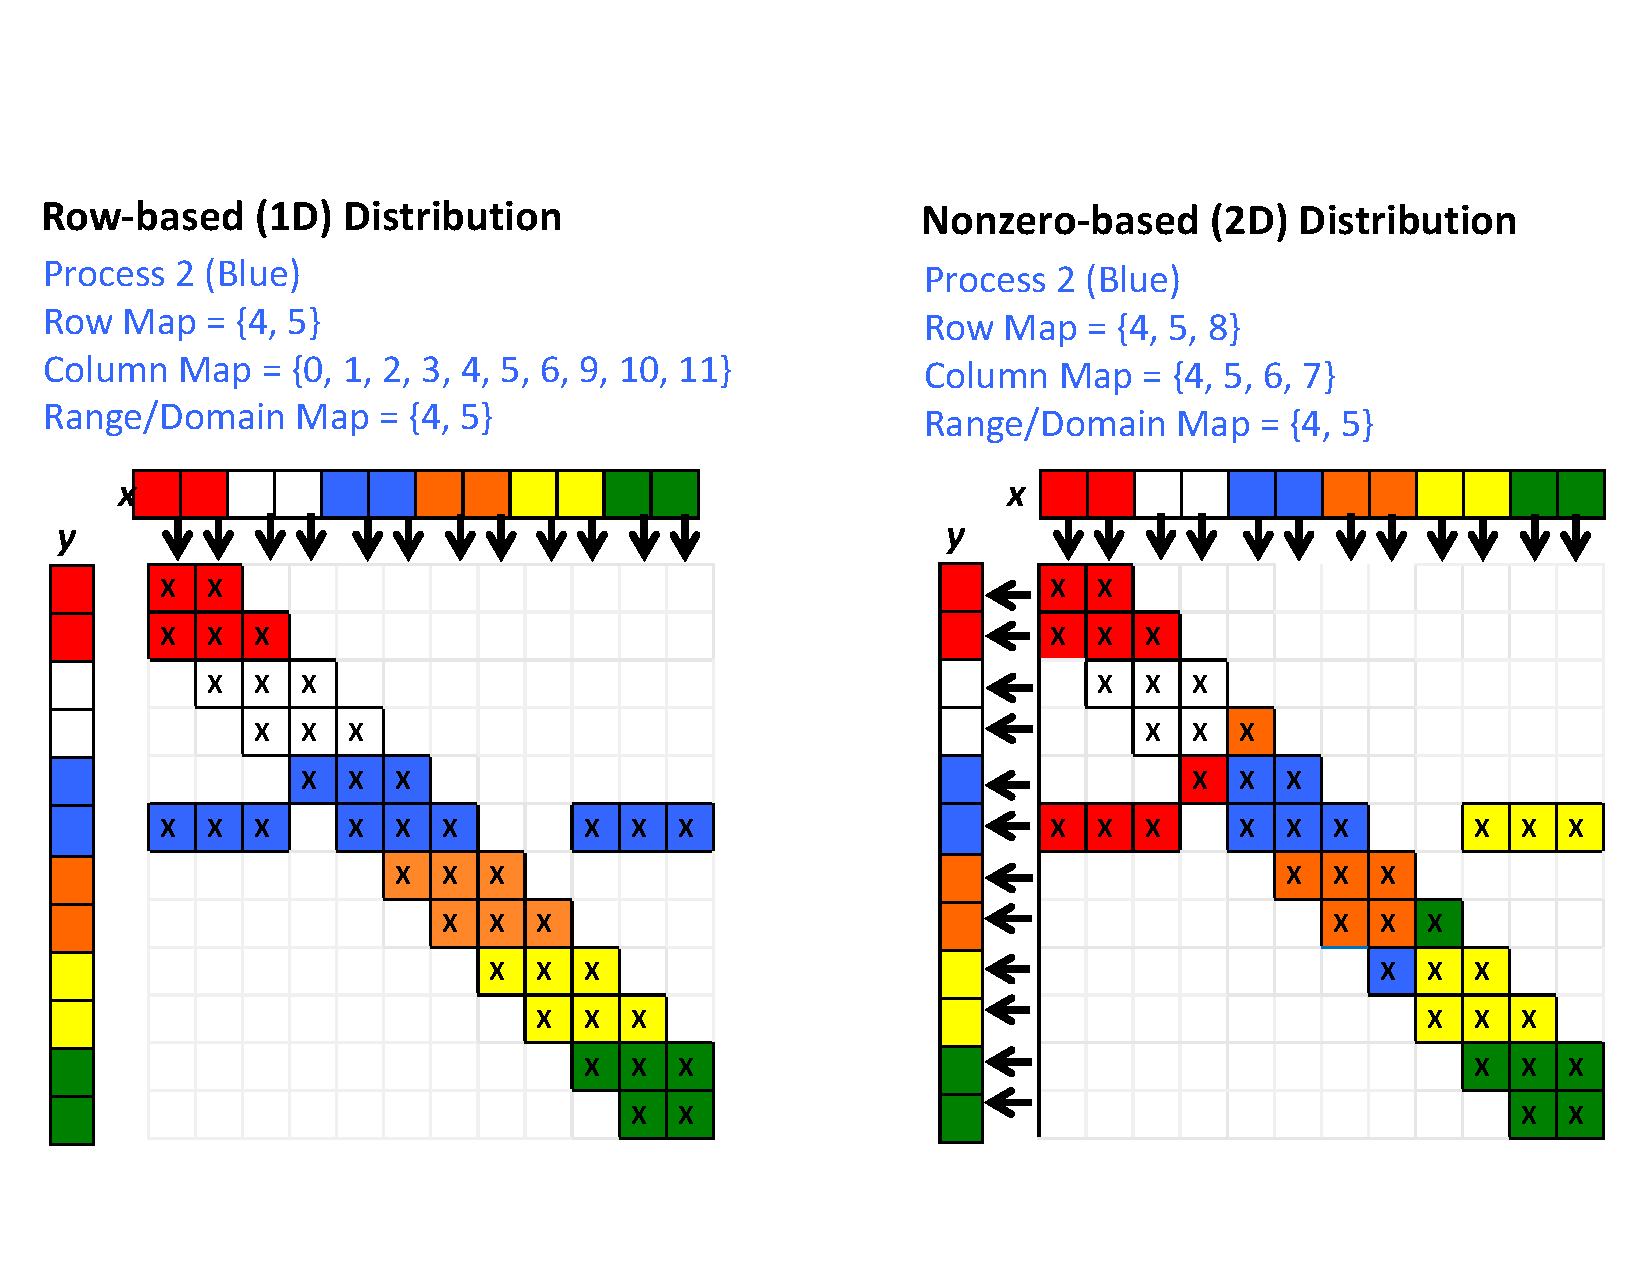
\includegraphics[keepaspectratio=true, width=6in]{figs/trilinosmaps}
   \caption[Examples of a distributed matrix and vectors in Trilinos]{Examples of a distributed matrix and vectors in Trilinos.  The left figure uses a row-based distribution; the right figure uses a nonzero-based distribution.  Colors indicate processor assignment.  The {\tt Map} entries for the blue processor are listed.}
   \label{fig:trilinosmap}
\end{figure}


\section{Tpetra MultiVectors} \label{sec:multivectors}

Tpetra's {\tt MultiVector} class contains $R$ vectors of length $n$, 
distributed to processors according to a Tpetra {\tt Map}.  In Figure
~\ref{fig:trilinosmap}, the input and output vectors $x$ and $y$ are 
{\tt MultiVectors} of length $n=12$ with $R=1$ vector.  They are distributed 
to six processors using ``one-to-one'' maps, so that each entry is uniquely
assigned to a processors.  {\tt MultiVectors} may also have maps that are 
``overlapped'' (not one-to-one) so that multiple processors have copies
of the vectors entries.  Such overlapped maps are used in sparse matrix-vector
multiplication (SpMV), where several processors may contribute to a
single output vector's entry.  (See Chapter~\ref{sec:mttkrp} for details.)
The {\tt MultiVector} class provides operations such as dot products, 
random vector generation, vector normalization, scaling, and vector norms.

\section{Trilinos Communication} \label{sec:import}

Trilinos' Teuchos package provides wrappers around MPI Communicators.
These wrappers allows Trilinos to be built with MPI for parallel execution,
or without it for serial execution.  They wrap the fundamental operations of
MPI (send, receive, reduce, gather), and are used in all of Tpetra's 
distributed objects.

Tpetra provides the class {\tt Import} to establish communication
patterns between pairs of maps.  For example, an {\tt Import} object can be used
to redistribute data from a source MultiVector using one map to a target 
Multivector using a different map.  They can reverse the communication pattern
as well, sending the data from the target object to the source.  Data can be
copied or accumulated into the target object; the latter allows data from
several sources to be added into a single target entry.  An {\tt Import} object
uses point-to-point communication in an underlying Tpetra {\tt Distributor}
class to perform communication.


    % !TEX root = 00_MAIN.tex

\chapter{GentenMPI classes} \label{sec:classes}

GentenMPI's tensor and factor matrix classes rely on the Tpetra classes 
described in Chapter~\ref{sec:trilinos}, with additional structures 
needed to support higher-order tensor data.

\section{Sparse tensor} \label{sec:sptensor}

{\bf File:  pt\_sptensor.hpp}

In GentenMPI's distributed sparse tensor class, each tensor nonzero is assigned
and stored on a single processor.  Tensor nonzeros are stored in coordinate
format; that is, a nonzero is represented by its global tensor indices
in each mode and its value.  A processor's nonzeros' indices and values are
stored in {\tt Kokkos::View} data structures, analogous to 2D and 1D arrays,
respectively.

For each tensor mode, the distributed tensor stores a Tpetra {\tt Map},
listing the indices in the mode for which a processor has nonzeros.  These
maps are analogous to the row and column maps stored for Tpetra matrices
(see Section~\ref{sec:maps}, and most closely resemble the overlapped
maps used for matrix
distributions (as in Figure~\ref{fig:trilinosmap}, right).  
For example, for a nonzero tensor entry $x_{ijk}$ in $\X$, 
index $i$ is in the mode-0 map, index $j$ is in the mode-1 map, and index
$k$ is in the mode-2 map.

Sparse tensors may also have bounding box information specified by a distributed sparse tensor bounding box class ({\bf File: pt\_sptensor\_boundingbox.hpp}).
In the case the tensor is distributed using a ``medium-grain'' distribution \cite{SK16}, for example, all of the processor's nonzero entries fall within a Cartesian product of mode index ranges.
These ranges can be stored as a bounding box, which is required for sampling strategies (see \Cref{sec:sampling}) within the GCP-SGD algorithm.

\section{Factor matrices} \label{sec:factormatrix}

{\bf File:  pt\_factormatrix.hpp}

A factor matrix $A \in \mathbb{R}^{I \times R}$ is a Tpetra {\tt MultiVector} 
of length $I$ with $R$ vectors (see Section~\ref{sec:multivectors}).  It 
exploits the MultiVector's methods for normalization, randomization,
and norm calculations, as well as the MultiVector's map for its distribution.
Like MultiVectors, factor matrices may be distributed uniquely (with 
one-to-one maps) or with copies (with overlapped maps).

By default, Tpetra stores the MultiVector data in column-major order
(Kokkos::LayoutLeft).  For many factor matrix operations, however, data is
more efficiently accessed row-wise --- that is, accessing 
all $R$ entries for a given index $i$.  Thus, GentenMPI modifies the 
Tpetra MultiVector to use row-major storage (Kokkos::LayoutRight).
Results showing the benefit of using row-major storage are in 
Chapter~\ref{sec:mttkrp}.

\section{Square local matrices} \label{sec:squarelocalmatrix}

{\bf File:  pt\_squarelocalmatrix.hpp}

A square local matrix $G\in \mathbb{R}^{R \times R}$ is stored redundantly on every processor as a \texttt{Kokkos::View} 2D data structure.
This class is used for Gram matrices of factor matrices and the temporary matrices computed from them.
Operations defined for square local matrices include Hadamard (elementwise) products with other square local matrices and with the outer product of a vector with itself and the sum of entries in the matrix (without absolute value).
These operations are useful in forming linear systems within CP-ALS iterations (see \Cref{sec:system}) and in computing the norm of a Kruskal tensor (see \Cref{sec:ktensor}), which itself is used in computing the 2-norm of the residual of a system (see \Cref{sec:system}).
Square local matrices are nearly always symmetric, but this symmetry is not exploited in the implementation (computations involving these small matrices are rarely a bottleneck).

\section{Kruskal tensor} \label{sec:ktensor}

{\bf File:  pt\_ktensor.hpp}

The distributed Kruskal tensor (ktensor) class contains a factor matrix for
each mode of the model $\M$, and an array $\lambda$ of length $R$~\cite{TTB_Sparse}.
%Each factor matrix 
Factor matrices stored in the ktensor use one-to-one maps; each factor
matrix entry is stored on only one processor. 
The $\lambda$ array is stored redundantly on every processor.

\section{System} \label{sec:system}

{\bf File:  pt\_system.hpp}

Many operations in tensor decomposition require both a sparse tensor and 
a Kruskal tensor.  GentenMPI's {\tt distSystem} class couples a sparse tensor
with a ktensor. 


A distSystem's sparse tensor provides Tpetra maps analogous to the row
and column maps of a Tpetra matrix. Its ktensor provides Tpetra maps 
analogous to the domain and range maps of a Tpetra matrix.  
The distSystem contains additional internal factor matrices for each mode, 
distributed according to the \emph{sparse tensor's} maps. These factor
matrices hold factor matrix entries corresponding to the stored 
nonzeros of the sparse tensor and typically have overlapped maps.
The internal factor matrix entries are used, for example, to evaluate
the model $\M$ at the indices of the sparse tensor.
To update the internal factor matrices, the distSystem uses
a Tpetra {\tt Import} object for each mode; the object contains the 
communication pattern necessary to transfer factor matrix entries from the
ktensor's distribution to these internal factor matrices, and vice versa.  

Operations requiring a sparse tensor and ktensor are also in the 
distSystem class.  These operations include CP-ALS, GCP-SGD, MTTKRP,
residual norm computation, loss function evaluation, and 
evaluation of the model $\T M$.

\section{Sampling Strategies} \label{sec:sampling}

{\bf File:  pt\_samplingstrategies.hpp}

The GCP-SGD algorithm \cite{KH19} can involve multiple sampling strategies of a sparse tensor (see \cref{sec:gcp_sample}).
SamplingStrategy is a base class with a derived class for each of three different strategies: stratified, semi-stratified, and full.
All of the sampling strategies involve only local data, even for the distributed implementation.
For all of the cases, the sampled entries are stored as a sparse tensor (see \cref{sec:sptensor}) with both nonzero and (sampled) zero values stored explicitly.
(Kolda~\cite{koldablog} uses the term ``scarce tensors'' to refer to sparse 
tensors storing both nonzeros and zeros as we do here.)

The stratified strategy samples nonzeros and zeros separately.
Nonzeros are sampled uniformly from the nonzeros in the original tensor, and zeros are sampled uniformly from within the full range of indices (in the distributed case, this range is determined by the bounding box of the sparse tensor, as described in \cref{sec:sptensor}).
In order to ensure that sampled zeros do not correspond to nonzero entries, each zero sample must be checked against the nonzero entries of the original tensor.
This is implemented using a hash: all original nonzero entries are hashed with a \texttt{Kokkos:UnorderedMap}\footnote{The TensorHash class ({\bf File: pt\_tensorhash.hpp}) wraps the \texttt{Kokkos:UnorderedMap} in order to use a variable number of indices (up to 6).}, and sampled zero indices are checked against the hash before being accepted as samples.

The semi-stratified strategy also samples nonzeros and zeros separately.
Again, nonzeros are sampled uniformly from the nonzeros in the original tensor, and zeros are sampled uniformly from within the bounding box.
In this case, zero samples are accepted whether or not they correspond to an original nonzero value; this possible inconsistency is accounted for within the GCP-SGD algorithm.

The full sampling strategy is used only for testing and debugging.
It samples all nonzero values and all zero values of the original tensor and stores them in sparse format.

\section{Loss Functions} \label{sec:lossfns}

{\bf File:  pt\_lossfns.hpp}

The Generalized CP (GCP) decomposition is defined for general loss functions.
The loss function can be specified by a derived class of the base lossFunction class.
The base class has three key operations: function evaluation, partial derivative evaluation, and model lower bound.
For example, for the $L^2$ loss function (for Gaussian data), the loss function evaluation returns $f(x,m) = (x-m)^2$, the partial derivative evaluation returns $\frac{\partial f}{\partial m}(x,m) = 2(x-m)$, and the model lower bound is $-\infty$ (implemented as the lowest floating point number).
The distributions with loss functions implemented are Gaussian, Poisson (-log), Bernoulli (odds and logit), Rayleigh, and Gamma. 


    % !TEX root = 00_MAIN.tex

\chapter{MTTKRP} \label{sec:mttkrp}

The Matricized Tensor Times Khatri-Rao Product (MTTKRP) operation is a key 
kernel of many tensor decomposition methods.  In CP-ALS, for example,
MTTKRP updates one factor matrix $A$ of a Kruskal tensor using values from
the other factor matrices $B$ and $C$ as follows:
\begin{equation}
\label{eq:mttkrp}
a_{ir} = \sum_{jk \in \X} x_{ijk} b_{jr} c_{kr}, \; i=1,\ldots,I, \; r=1,\ldots,R
\end{equation}

In GCP-SGD, MTTKRP updates factor matrices of a gradient ktensor $\T G$ in a 
similar manner.

\section{Parallel MTTKRP vs. Parallel SpMV} \label{sec:spmv}

The analogy between parallel MTTKRP and parallel sparse matrix-vector
multiplication (SpMV) is strong.   In the SpMV $(\vec a) = X (\vec b)$, 
vector entries of the vector $(\vec a)$ are updated using the values 
of $(\vec b)$:
\begin{equation}
\label{eq:spmv}
a_i = \sum_{j \in \X} x_{ij} b_j.
\end{equation}
 
In parallel SpMV, input vector entries $b_j$ must be communicated to processors 
having nonzeros in column $j$ of the matrix; 
this communication is called an ``expand''
communication.  
The received values are multiplied by the processor's $x_{ij}$.
The resulting products are then summed across matrix rows.
All processors with nonzeros in row $i$ must accumulate their partial
sums into output vector entry $a_i$; this communication operation is 
called a ``fold'' communication.  These expand and fold operations are 
illustrated in Figure~\ref{fig:spmv}.

\begin{figure}[ht]
   \centering
   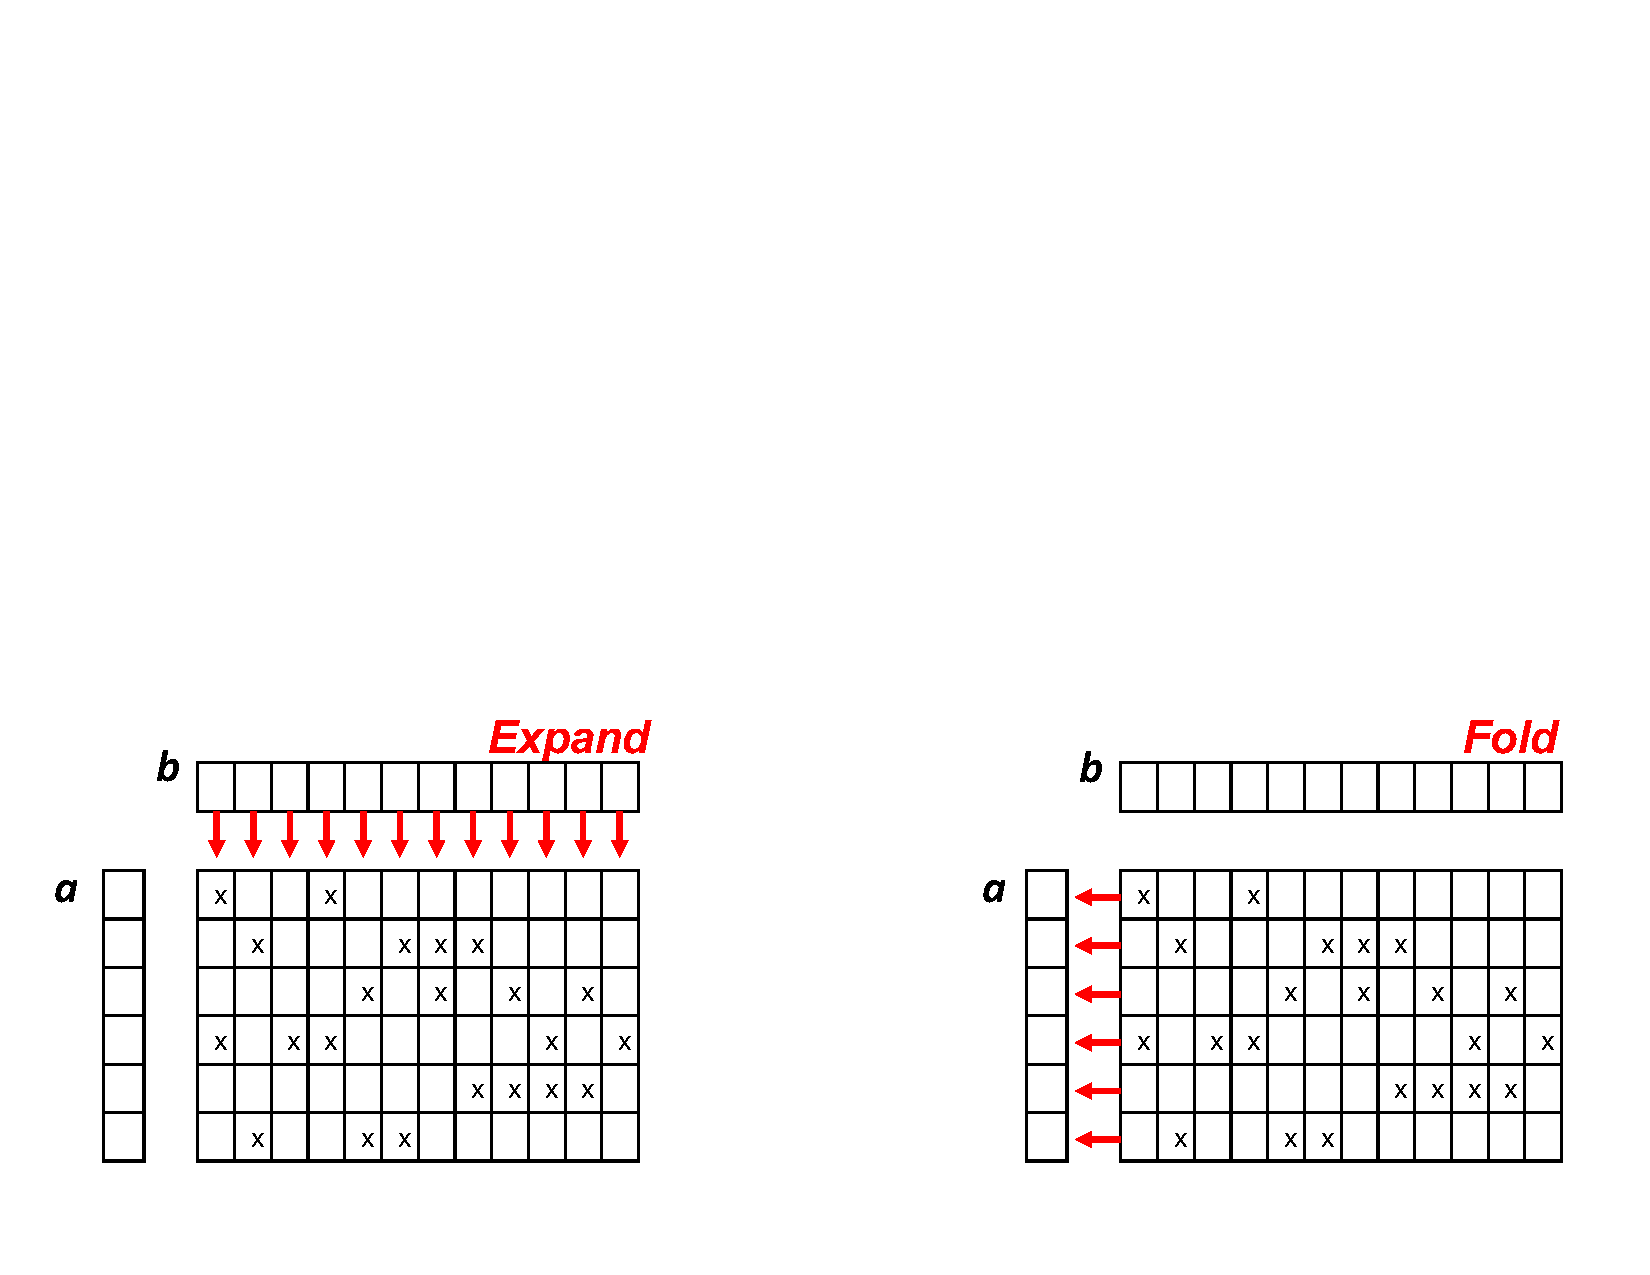
\includegraphics[keepaspectratio=true, width=6.5in]{figs/spmv}
   \caption[The expand and fold communication involved in SpMV]{The expand and fold communication involved in SpMV.  In the expand communication, the input vector entries $b_j$ are communicated to processors with nonzeros in column $j$.
Local products $x_{ij} b_j$ are computed. Then the fold communication 
accumulates partial sums across processors sharing matrix rows $i$ into output
vector entry $a_i$.}
   \label{fig:spmv}
\end{figure}

Parallel MTTKRP requires the same expand and fold communications, as 
illustrated in Figure~\ref{fig:mttkrp}.  In the expand communication,
entries from
factor matrices $B$ and $C$ are communicated to processors with 
corresponding tensor entries.  
Partial sums are then computed within the processor.  
The fold operation then communicates and accumulates
the partial sums into the result factor matrix $A$.

\begin{figure}[ht]
   \centering
   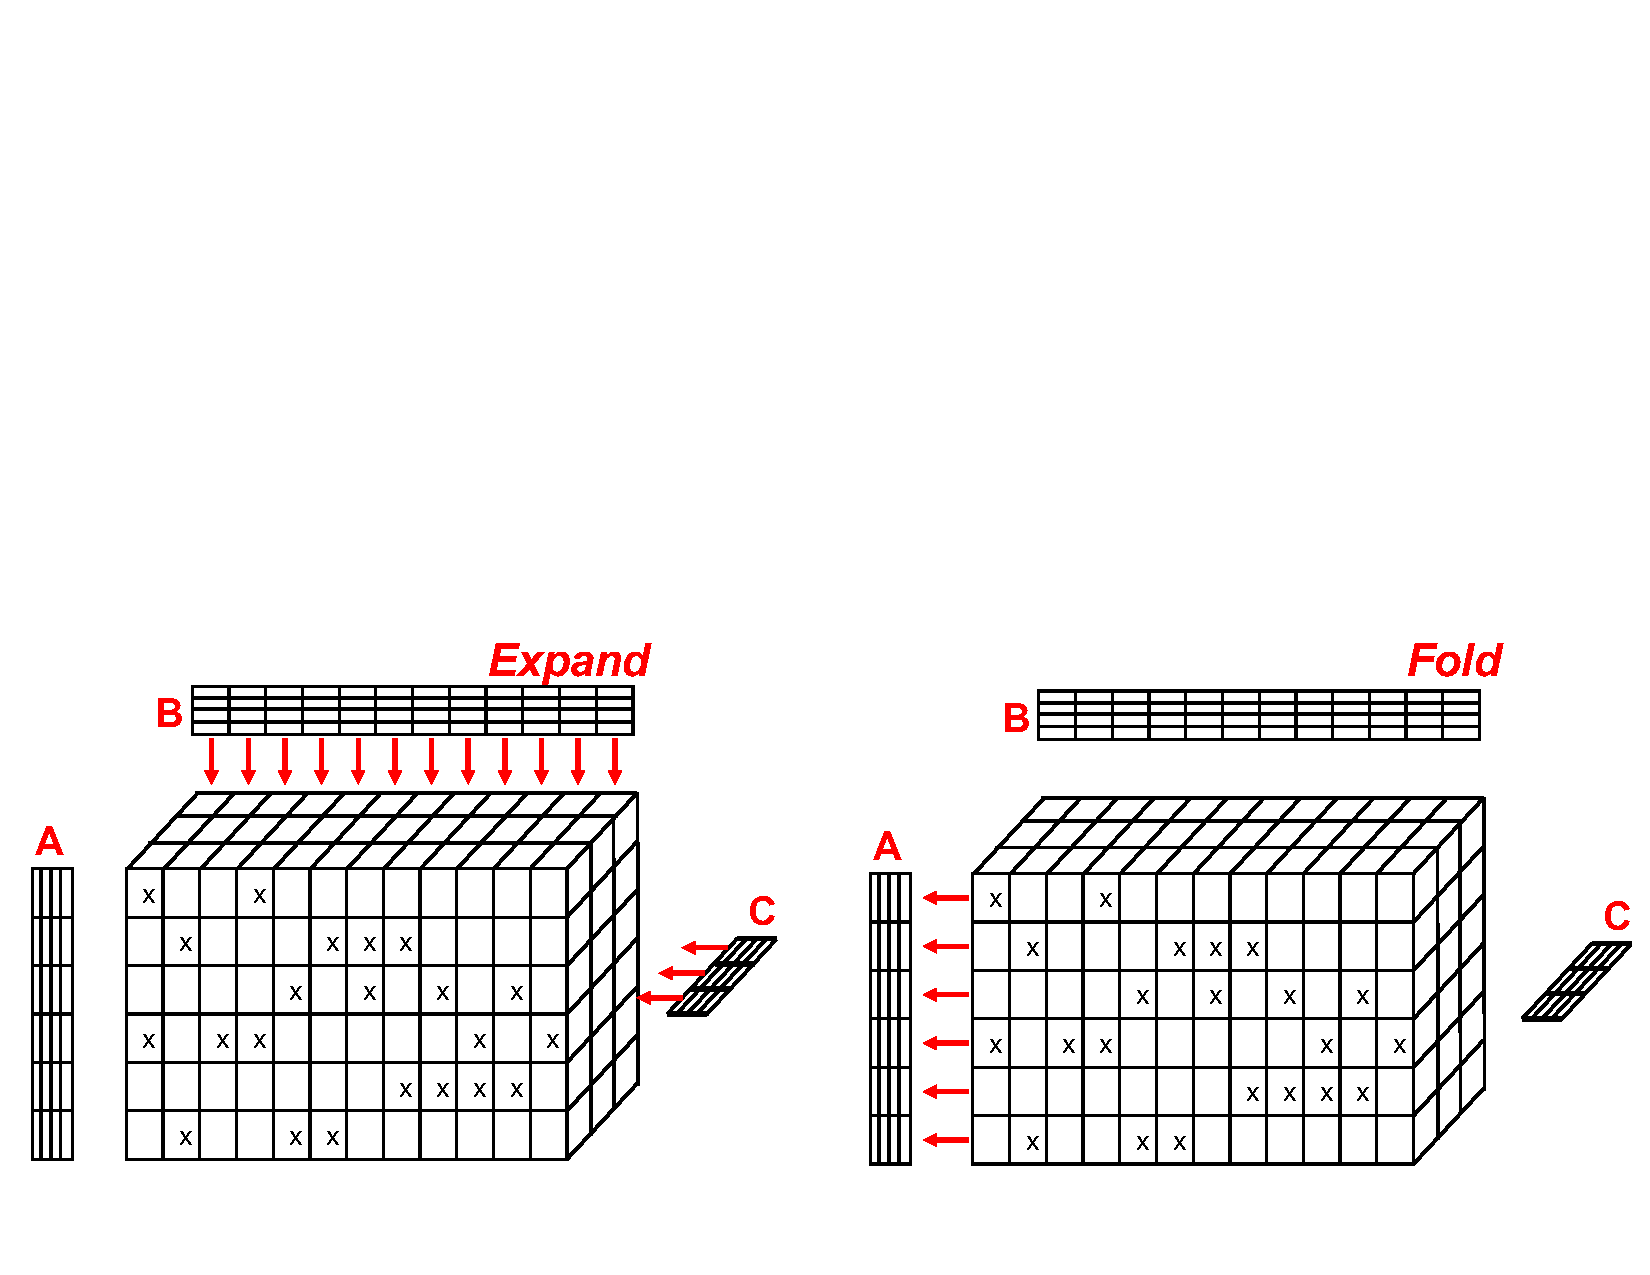
\includegraphics[keepaspectratio=true, width=6.5in]{figs/mttkrp}
   \caption[The expand and fold communication involved in MTTKRP]{The expand and fold communication involved in MTTKRP.  In the expand communication, the entries input factor matrices $B$ and $C$ are communicated to processors with corresponding entries in the tensor $\X$.
Local products $x_{ijk} b_{jr} c_{kr}$ are computed. 
Then the fold communication 
accumulates partial sums across processors into output
factor matrix $A$.}
   \label{fig:mttkrp}
\end{figure}


\section{Implementation}

The MTTKRP implementation in GentenMPI works much like the implementation 
of SpMV in Tpetra.  Here, we'll assume factor matrix $A$ will receive the 
result of the MTTKRP computed from three-way tensor $\X$ and 
factor matrices $B$ and $C$; this scenario is relevant to CP-ALS 
(Chapter~\ref{sec:cpals}).

\begin{enumerate}
\item MTTKRP requires a {\tt distSystem} object $D$ constructed from the tensor
$\X$ and a Kruskal tensor with the factor matrices $A$, $B$, and $C$.  
During construction of the $D$, its internal factor matrices $\hat A$, 
$\hat B$, and $\hat C$ are updated 
via communication using the {\tt Import} objects in each mode.
This update constitutes the ``expand'' communication, and brings to each 
processor the factor matrix entries in each mode corresponding to the 
indices of the processor's $x_{ijk}$ entries.

\item \label{mttkrp:local} Local products are computed within each processor.  The processor loops
over its owned tensor entries $x_{ijk}$ and multiplies them by the associated
entries $\hat b_{jr}$ and $\hat c_{kr}$, accumulating the results in 
$\hat a_{ir}$.  This operation is a triply nested loop, first over the 
$N_p$ tensor entries on a processor, 
then over tensor modes, and then over the rank $R$.

\item \label{mttkrp:fold} After completion of the local computation, $D$'s {\tt Import} object 
associated with $A$ communicates values from $\hat A$ 
back to $A$, with contributions from multiple 
processors summed into $A$.  This operation is the ``fold'' communication.

\item \label{mttkrp:lastupdate} Once $A$ is updated by all processors, 
the accrued values of $A$ can be communicated back to $\hat A$ to keep the 
internal factor matrices up-to-date with actual factor matrix values.
\end{enumerate}

For GCP-SGD (Chapter~\ref{sec:gcp}), 
the result of the MTTKRP with $B$ and $C$ is not stored in 
$A$, but rather, is stored in an additional factor matrix $G$.  In this case,
additional storage $\hat G$ is used to receive the result of the MTTKRP in
step~\ref{mttkrp:local}, and $\hat G$ is communicated to $G$ in 
step~\ref{mttkrp:fold}.  Step~\ref{mttkrp:lastupdate} is not needed since
neither $\hat A$ nor $A$ is changed in the MTTKRP.

\section{Column-major vs Row-major}

The default layout of data in Tpetra's {\tt MultiVector} class
is column-major ({\tt Kokkos::LayoutLeft}); that is, for an $I \times R$ factor 
matrix, the first vector of length $I$ is stored, followed by the second
vector of length $I$, and so on.  This layout is convenient for some linear
solvers that need to access a single vector or a subset of vectors of a 
given multivector.
However, in MTTKRP, all $R$ factor matrix
entries for a given index $i$ are accessed together in step~\ref{mttkrp:local} 
above.  The default layout causes strided memory acceses that can lead to 
poor cache performance.

A better layout for MTTKRP is row-major ({\tt Kokkos::LayoutRight}), in
which all $R$ entries for a given index $i$ are stored contiguously in 
memory.  Thus, GentenMPI uses a modified Tpetra {\tt MultiVector} that 
uses row-major storage; these modifications were trivial and did not interfere
with Tpetra's communication of multivector data values.

Figure~\ref{fig:layouts} shows the difference in performance using 
column-major vs row-major layouts.  This example was run on one processor
of Sandia's SkyBridge cluster with 2.6GHz Intel Sandy Bridge processors.
It uses the \emph{delicious-4d} tensor from the FROSTT~\cite{FROSTT} tensor collection,
a $532,924 \times 17,262,471 \times 2,480,308 \times 1443$ tensor with 140 million
nonzeros.  With rank $R=8$, the difference in MTTKRP time between column-
and row-major layouts is visible; column-major layout requires 1.7 times more
execution time per MTTKRP.  With larger values of
$R$, the difference becomes even more significant, with column-major layout
taking 3.4 times longer than row-major layout for $R=32$.


\begin{figure}[ht]
   \centering
   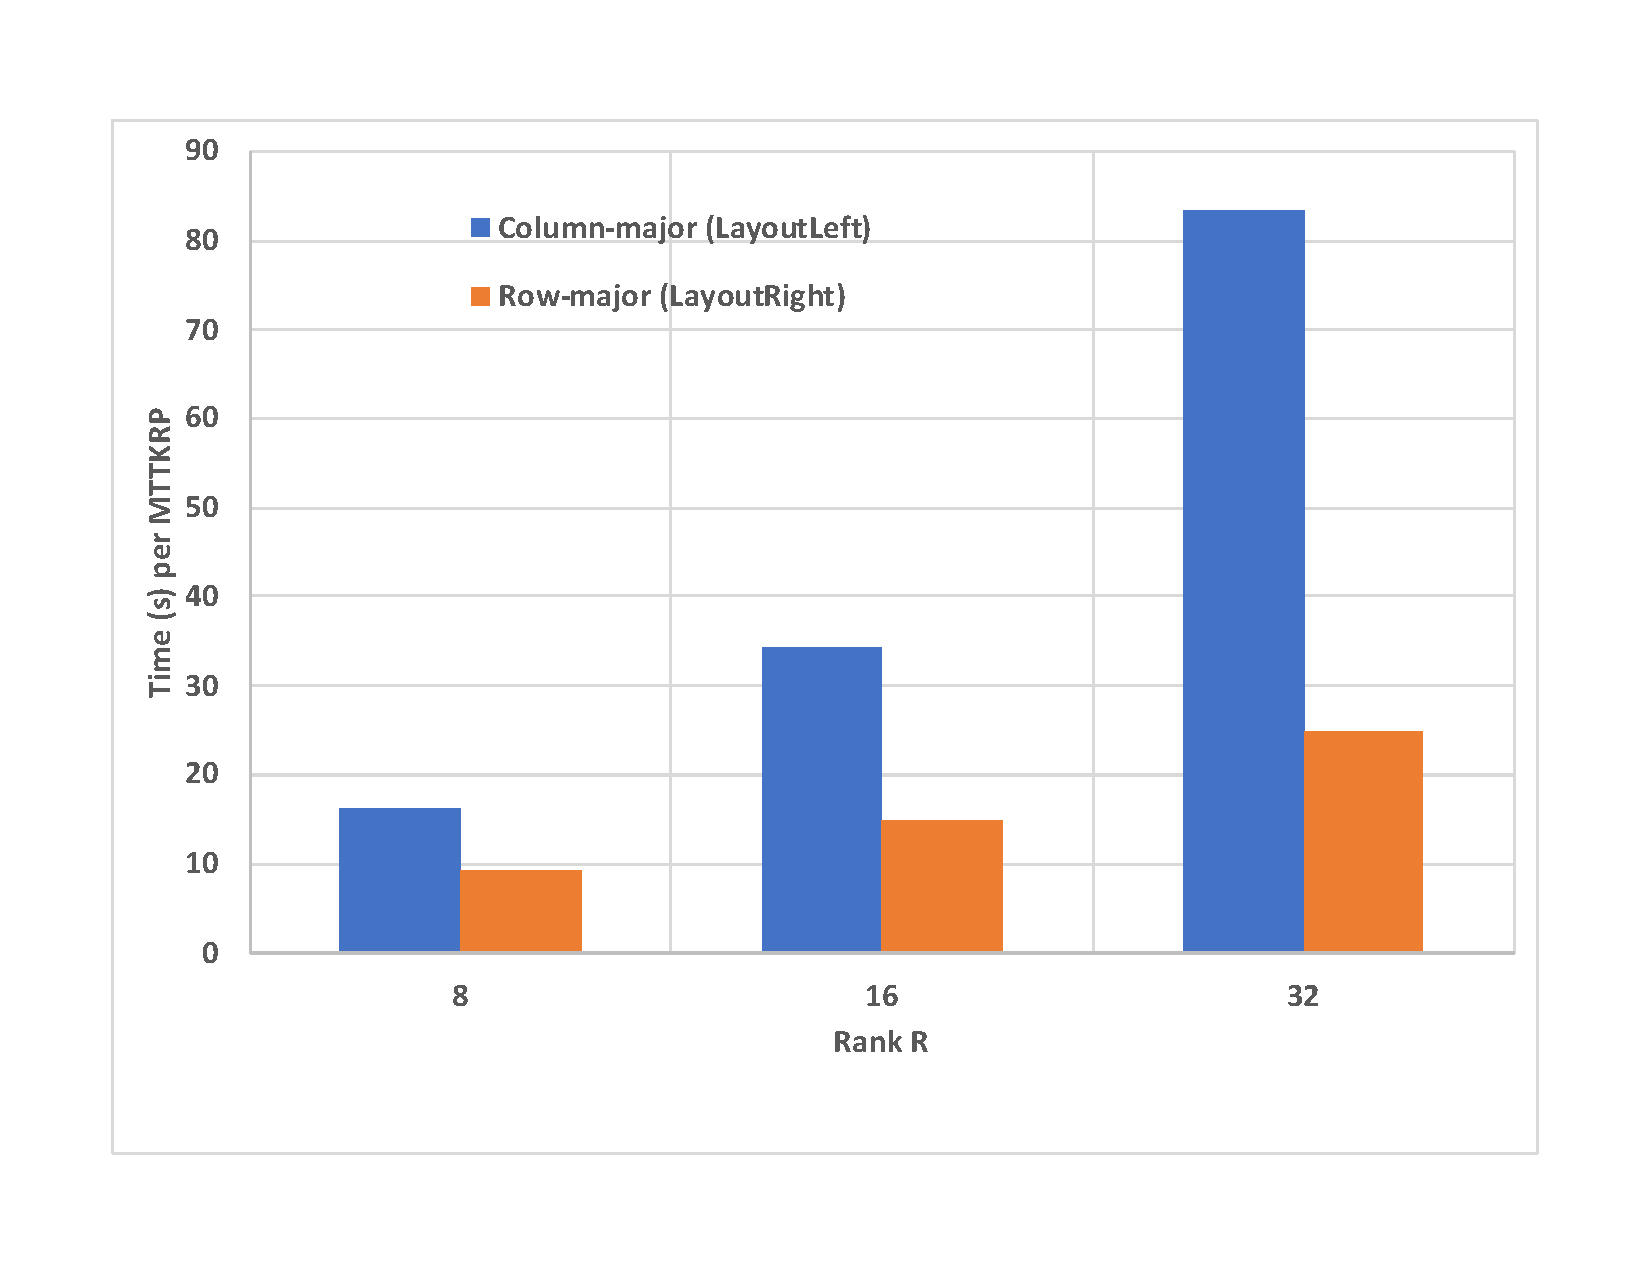
\includegraphics[keepaspectratio=true, width=4.5in]{figs/layouts}
   \caption[MTTKRP times using column- and row-major layout of factor matrices]{MTTKRP times using column-major (LayoutLeft) and row-major
(LayoutRight) layout of the factor matrices. (\emph{delicious-4d}
tensor, rank $R=8,16,32$)}
   \label{fig:layouts}
\end{figure}

For all experiments in the remainder of this report, GentenMPI uses
row-major (\texttt{Kokkos::LayoutRight}) layout for all factor matrices.

    % !TEX root = 00_MAIN.tex

\chapter{CP-ALS} \label{sec:cpals}

The Canonical Polyadic decomposition (CPD)~\cite{CC70,Harshman70}
is a tensor decomposition that uses an $L^2$ loss function
$f(x,m) \equiv (x-m)^2$ in the optimization in Equation~\ref{eq:gcp}.
CP-ALS --- CP solved via alternating least squares optimization ---
is one approach for performing this tensor decomposition.

\section{Algorithm} \label{sec:cpals_alg}

CP-ALS uses an alternating least squares approach to perform
the optimization. A sketch of the algorithm for three-way tensors 
is included in Algorithm~\ref{alg:cpals}. The method and GentenMPI 
implementation extend to tensors
of any order; for more details, see Kolda and Bader's
survey~\cite{KB09}.  First, factor matrix $A$ is computed with fixed 
factor matrices $B$ and $C$; then $B$ is updated using $A$ and $C$; and
then $C$ is updated using $A$ and $B$.  The algorithm iterates over the 
updates until a desired convergence tolerance is reached or the specified
maximum numer of iterations is exceeded.


\begin{algorithm}
  \caption{CP-ALS algorithm for a three-mode tensor $\X$}
  \label{alg:cpals}
  \begin{algorithmic}[1]
    \Procedure{CP-ALS}{$\X, [\lambda;A,B,C]$}
    \Repeat{}
      \State $A \gets $ MTTKRP($\X,B,C$) $(C^T C * B^T B)^{-1}$
      \State Normalize columns of $A$
      \State $B \gets $ MTTKRP($\X,C,A$) $(A^T A * C^T C)^{-1}$
      \State Normalize columns of $B$
      \State $C \gets $ MTTKRP($\X,A,B$) $(B^T B * A^T A)^{-1}$
      \State Normalize columns of $C$; store norms as $\lambda$
    \Until{converged or max iterations reached}
    \State \Return{$[\lambda;A,B,C]$}
    \EndProcedure
  \end{algorithmic}
\end{algorithm}


\section{Implementation} \label{sec:cpals_impl}

In GentenMPI, CP-ALS is implemented using the MTTKRP algorithm described
in Chapter~\ref{sec:mttkrp}.  The $R \times R$ Gram matrices $(C^T C * B^T B)$
are small enough to replicate on every processor; contributions from each
processor are accumulated using an MPI\_Allreduce operation.  The 
linear systems involving these matrices are solved using LAPACK's GESV method.
Convergence is checked by computing the $L^2$-norm of $\X - \M$.

While GentenMPI's CP-ALS can function with any distribution of the tensor
and factor matrices, faster performance and better scaling is achieved when
the number of tensor entries per processor is balanced and tensor indices
are localized to reduce the number of factor matrix entries needed in MTTKRP.
The SPLATT tensor code provides a ``medium-grain'' decomposition in which
the tensor is divided into subtensors with roughly uniform number of 
nonzeros per subtensor~\cite{SK16}. 
In each mode, then, expand and fold communication is done among 
processors within a slice of subtensors.
A illustration of a medium-grain decomposition is in Figure~\ref{fig:medgrain}.
For a three-way tensor, $P=48$ processors are organized into a three-way 
$6 \times 4 \times 2$ grid.  
Cuts in each mode then greedily assign tensor slices to processors in a way
that balances the number of nonzero entries.

\begin{figure}[ht]
   \centering
   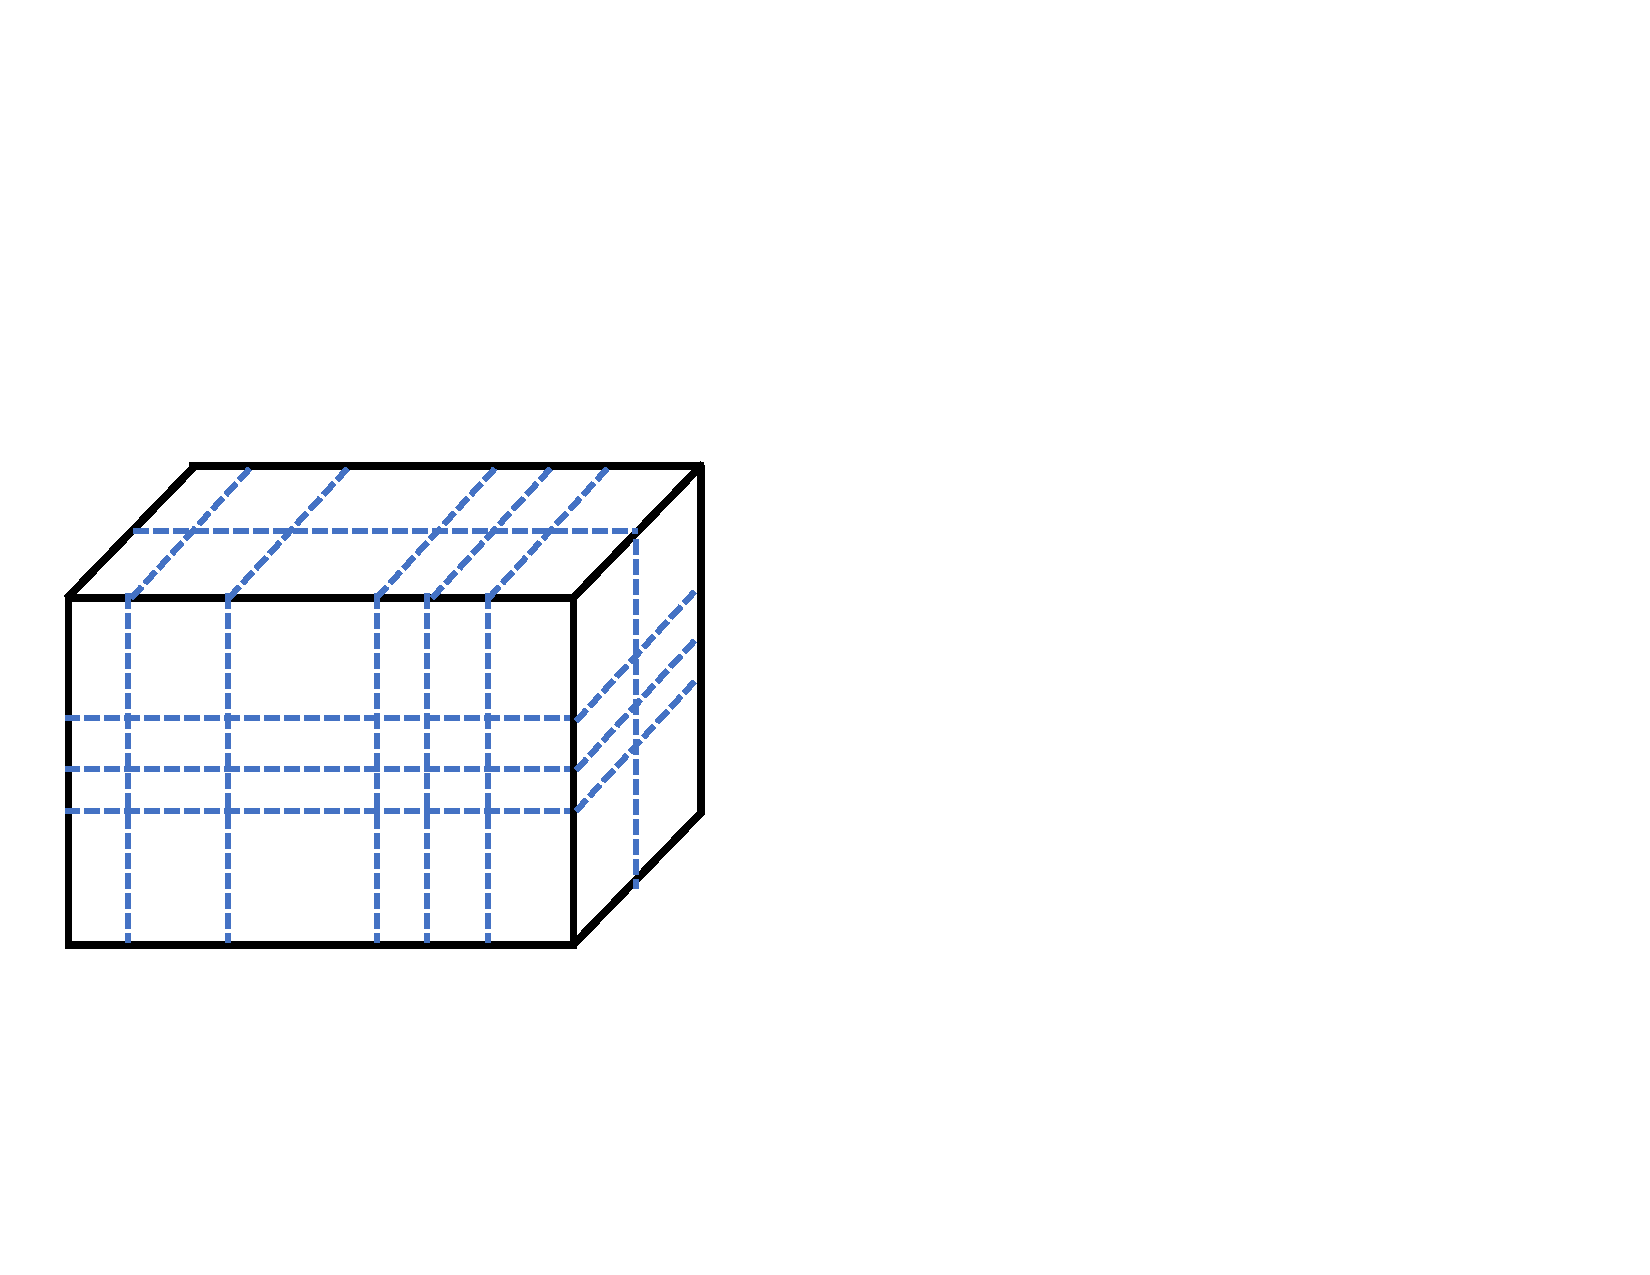
\includegraphics[keepaspectratio=true, width=2.5in]{figs/medgrain}
   \caption[SPLATT medium-grain distribution]{Illustration of a 
 SPLATT medium-grain distribution~\cite{SK16}
 of a three-way tensor to 48 processors}
   \label{fig:medgrain}
\end{figure}

We adopt this medium-grain decomposition for CP-ALS in GentenMPI. Because equal
number of nonzers are assigned to each processor, this decomposition 
provides good load balance in the MTTKRP computation.  While it doesn't 
explicitly attempt to minimize communication during MTTKRP, it provides 
reasonable alignment between factor matrix distributions and needed tensor 
entries.  And it is inexpensive to compute compared to partitions that 
do explicitly attempt to reduce communication, such as the hypergraph methods
of Kaya and Ucar~\cite{KayaUcarSC15}.

We use
the default Trilinos {\tt Map} layout (Section~\ref{sec:maps})
for factor matrices; that is, on $P$ processors,
factor matrix $A \in \mathbb{R}^{I \times R}$ is divided into $P$ chunks
of length $I/P$, with processor 0 receiving chunk \{$1,2,\ldots,I/P$\},
processor 1 receiving chunk \{$I/P+1,\ldots,2I/P$\}, and so on.


\section{Experimental Results} \label{sec:cpals_exp}

The main motivation in creating GentenMPI is to enable decomposition of
tensors too large to fit into a single node's memory.  To demonstrate this
capability, we study the weak-scaling of GentenMPI's CP-ALS by 
generating random sparse tensors and apply CP-ALS to them.  The generated
tensors are four-way tensors with 64 million nonzeros per processor and the 
mode lengths adjusted to maintain constant nonzero density of 0.001024.
With these characteristics, the tensor size is 12.6 Terabytes on 8192
processors:  524 billion nonzeros with four integers and one double per nonzero.

Weak scaling results on Sandia's SkyBridge cluster (2.6 GHz Intel Sandy
Bridge nodes with Infiniband network) are shown in Figure~\ref{fig:huge}.
We show both the average time per CP-ALS iteration and MTTKRP within a 
CP-ALS iteration.  Clearly, the MTTKRP kernel dominates the CP-ALS computation.
Weak scaling is very good, but degrades slightly due to an increased number
of neighboring processors (and, thus, of messages) as the number of 
processors increases. (Envision more layers of processors being added to
the processor distribution in Figure~\ref{fig:medgrain} as the number of 
processors increases.)


\begin{figure}[ht]
   \centering
   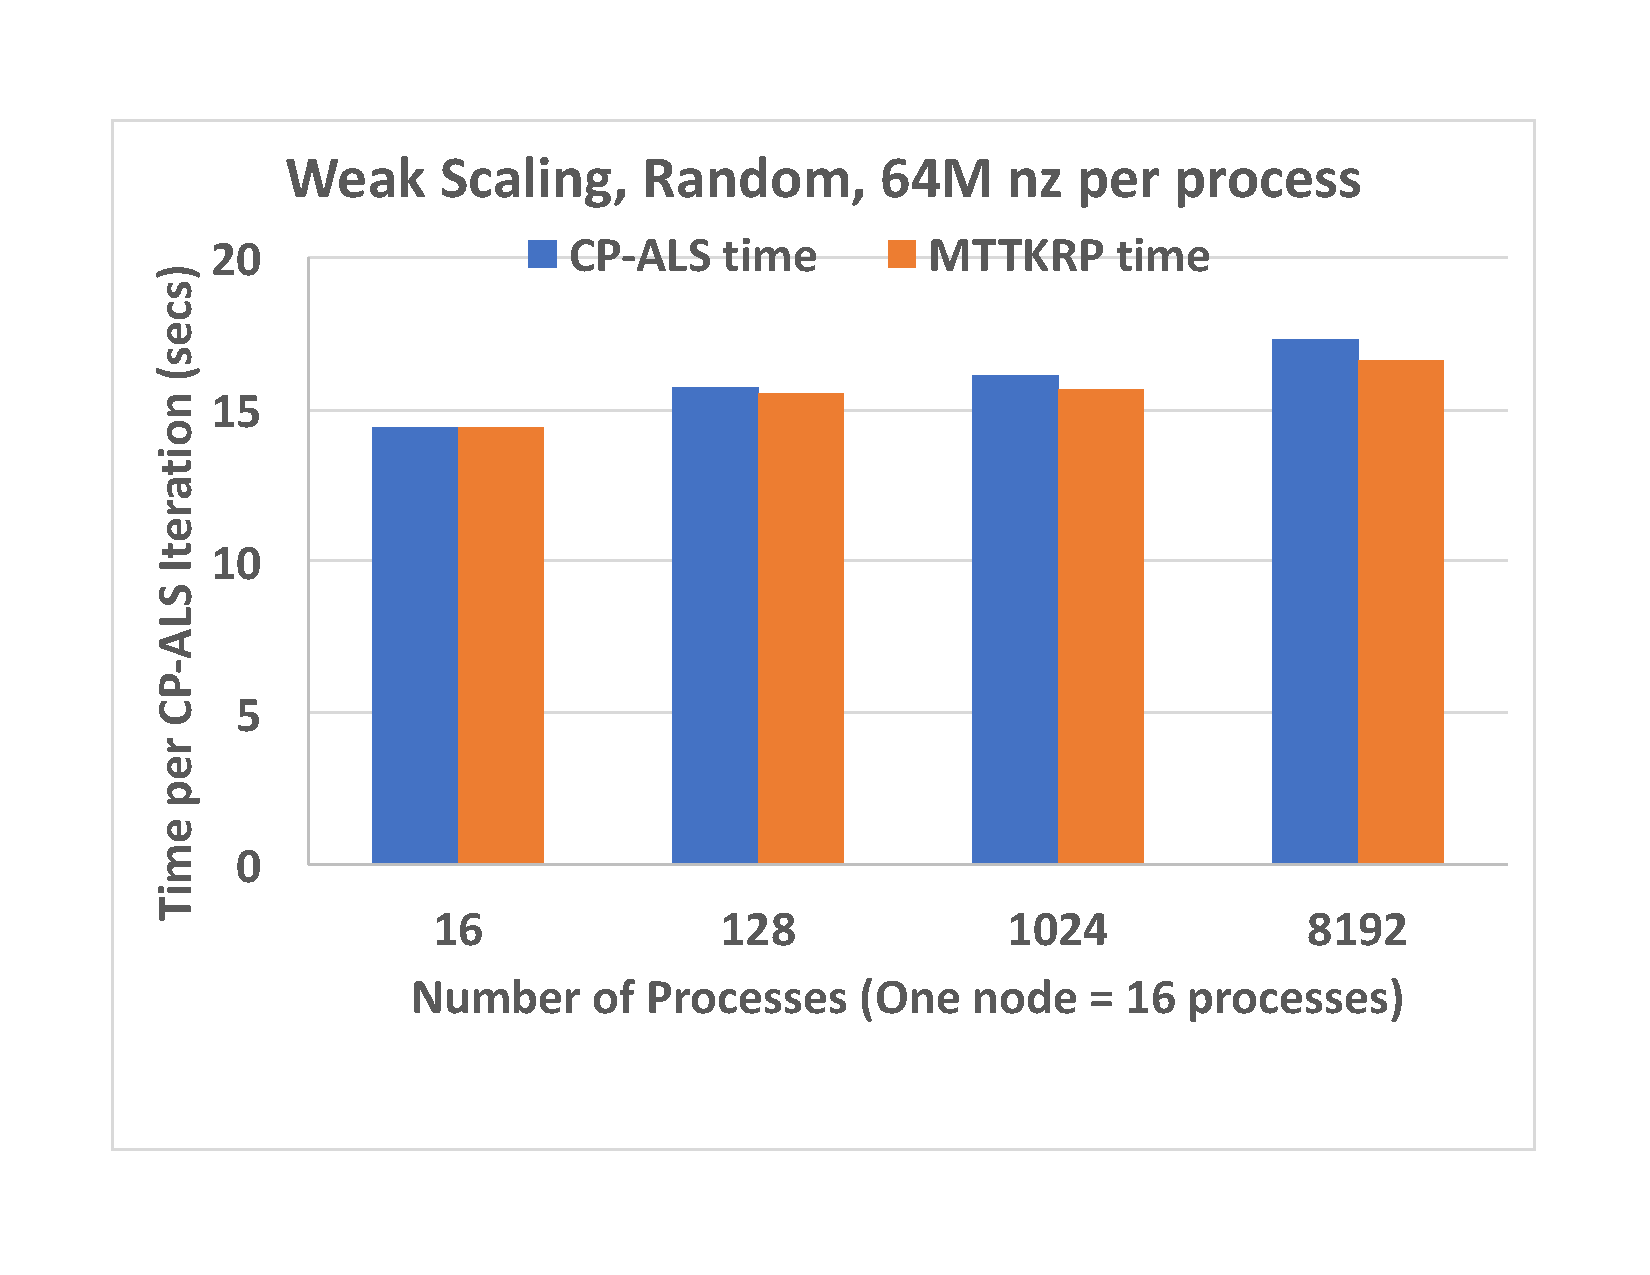
\includegraphics[keepaspectratio=true, width=4.5in]{figs/huge}
   \caption[Weak scaling of CP-ALS]{Weak scaling of CP-ALS on a four-way random tensor:  the time for one CP-ALS iteration is in blue, with the MTTKRP time per iteration in orange.
The largest tensor, decomposed on 8192 processors, is 12.6 Terabytes.}
   \label{fig:huge}
\end{figure}



We next examine the strong scaling of GentenMPI's CP-ALS implementation,
comparing GentenMPI's performance with SPLATT~\cite{SK16} and 
Genten~\cite{PK19}.
SPLATT can run with distributed memory parallelism only (``MPI-only'') or
with hybrid distributed memory and shared memory threading (``MPI+OpenMP'').
We compare with both configurations.  
For the MPI-only case, we use the same number of 
MPI ranks for SPLATT and GentenMPI.  For MPI+OpenMP, we use 16 threads per 
MPI rank and one MPI rank in SPLATT for every 16 MPI ranks in GentenMPI.
For 16 processor runs, we compare with Genten with 16 threads.

We begin with the \emph{delicious-4d} tensor from the FROSTT~\cite{FROSTT} 
tensor collection,
a $532,924 \times 17,262,471 \times 2,480,308 \times 1443$ tensor with 140 million
nonzeros.
We run with 16 to 1024 cores, with rank $R$ ranging from 8 to 128.
Times per CP-ALS iteration are shown in Figure~\ref{fig:cpals_delicious}.
We see that the strong scaling of GentenMPI is good in all experiments.
Runtimes are generally faster than SPLATT MPI-only; multithreading does
make SPLATT's performance with MPI+OpenMP superior to GentenMPI.
GentenMPI's runtimes are acceptable when compared to Genten.  GentenMPI
has the benefit that it can access sufficient memory for the $R=128$ case,
while Genten has the advantage that it can run on both multithreaded CPUs and 
GPUs.

\begin{figure}[ht]
   \centering
   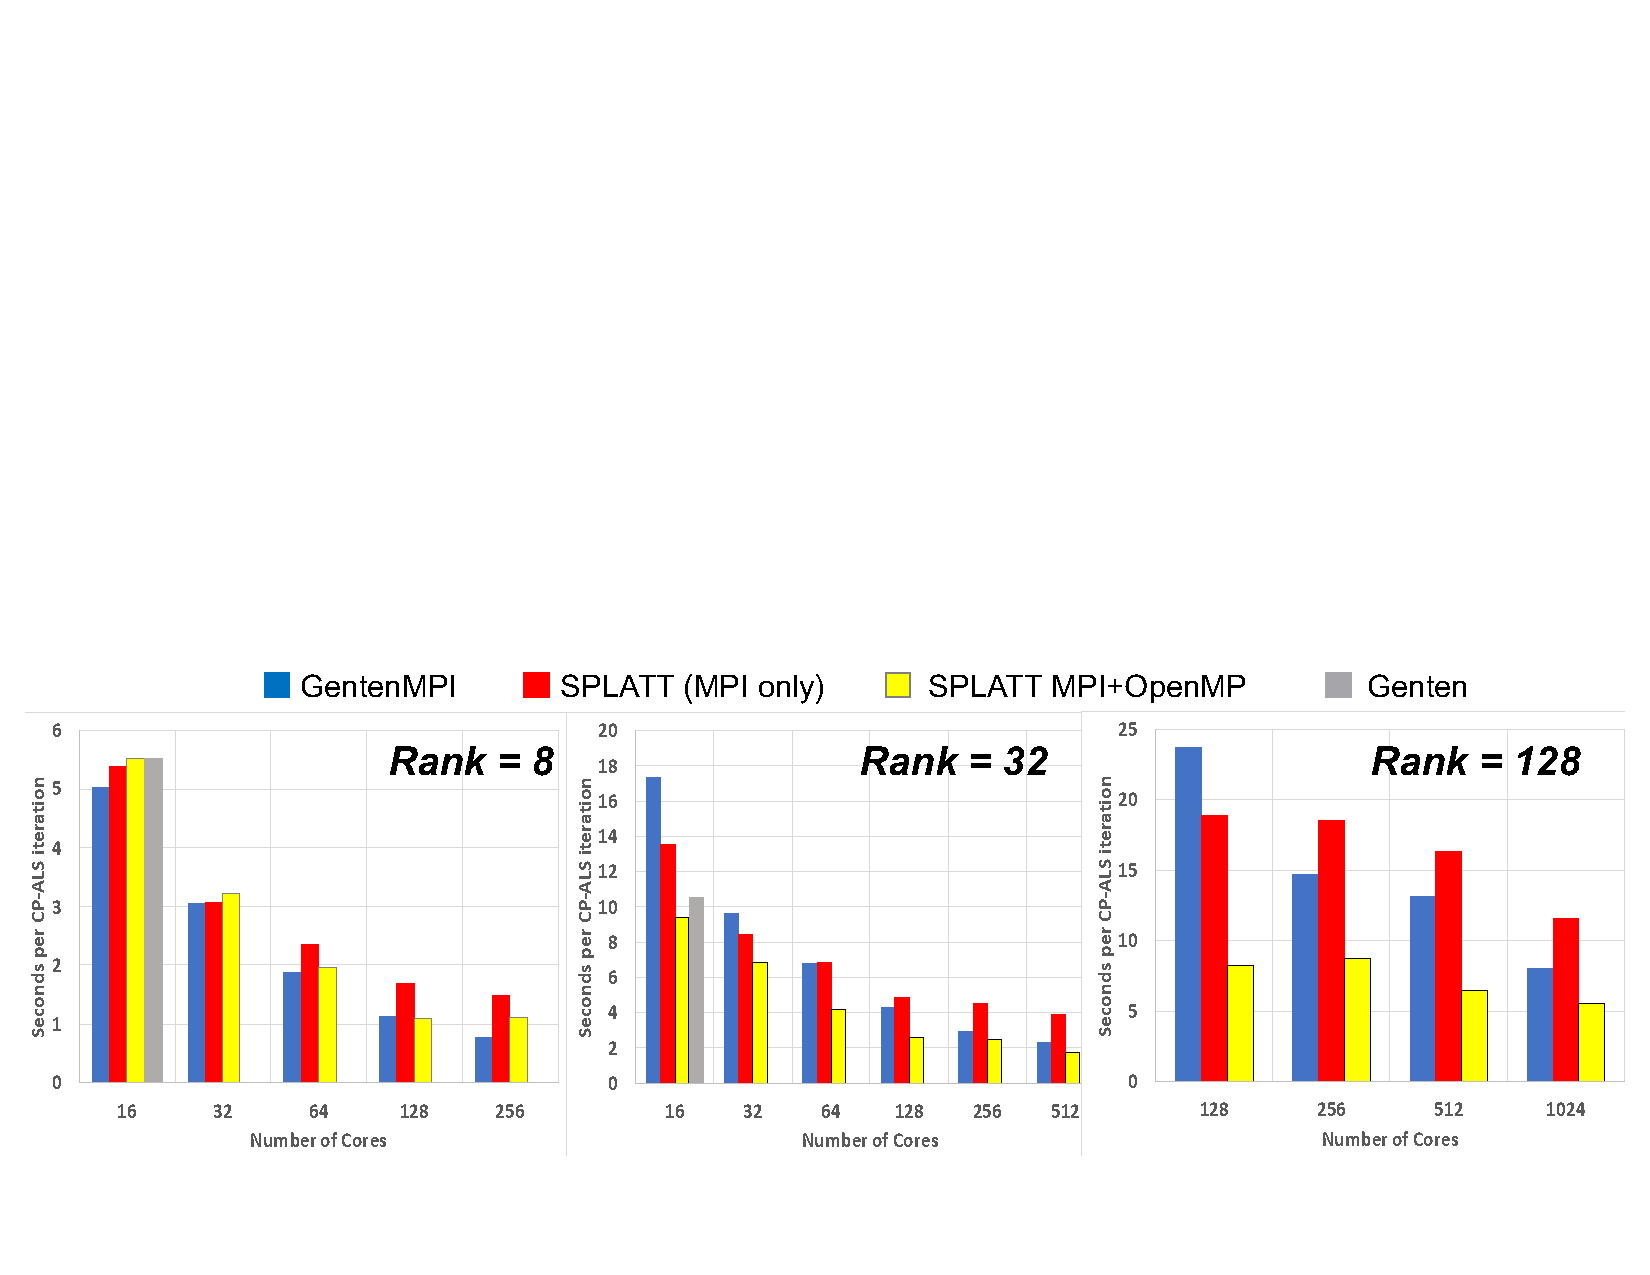
\includegraphics[keepaspectratio=true, width=6in]{figs/cpals_delicious}
   \caption[Strong scaling of CP-ALS on \emph{delicious-4d} tensor]{Strong scaling of CP-ALS on the \emph{delicious-4d} tensor from the FROSTT~\cite{FROSTT} collection.  GentenMPI times per CP-ALS iteration are compared
with those from Genten~\cite{PK19} and SPLATT~\cite{SK16} with MPI-only and MPI+OpenMP.}
   \label{fig:cpals_delicious}
\end{figure}



We demonstrate GentenMPI on the larger \emph{amazon-reviews} tensor from FROSTT,
a $4.8M \times 1.8M \times 1.8M$ tensor with 1.7 billion nonzeros.  This tensor is 
too large to fit in a single node of SkyBridge, so comparisons with Genten
are not possible.  For this tensor, we see in Figure~\ref{fig:cpals_amazon}
that GentenMPI's implementation is
faster than both SPLATT MPI-only and SPLATT MPI+OpenMP.  Strong scaling is 
good out to 1024 cores.

\begin{figure}[ht]
   \centering
   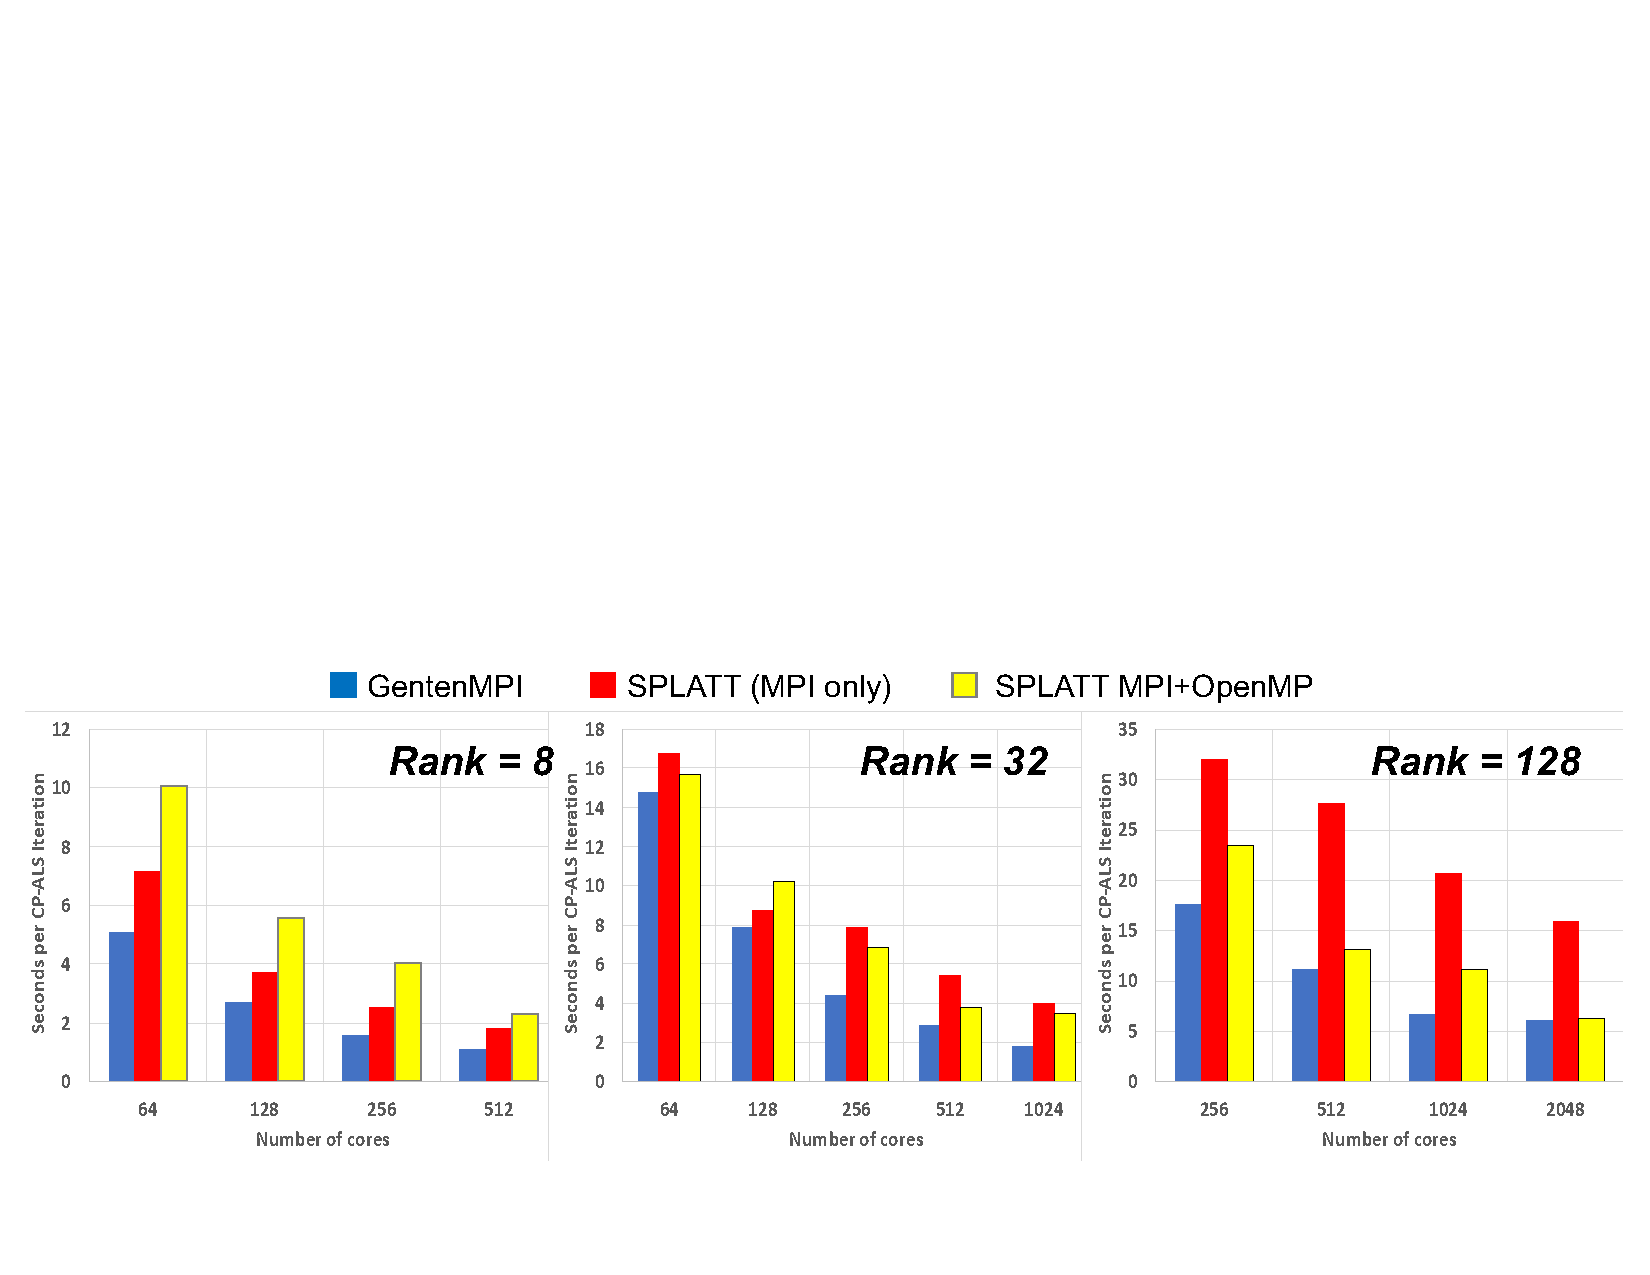
\includegraphics[keepaspectratio=true, width=6in]{figs/cpals_amazon}
   \caption[Strong scaling of CP-ALS on \emph{amazon-reviews} tensor]{Strong scaling of CP-ALS on the \emph{amazon-reviews} tensor from the FROSTT~\cite{FROSTT} collection.  GentenMPI times per CP-ALS iteration are compared
with those from SPLATT~\cite{SK16} with MPI-only and MPI+OpenMP.}
   \label{fig:cpals_amazon}
\end{figure}



    % !TEX root = 00_MAIN.tex

\chapter{GCP-SGD} \label{sec:gcp}

Kolda and Hong~\cite{KH19} propose using a stochastic gradient
descent method to solve the Generalized Canonical Polyadic (CP)
optimization of Equation~\ref{eq:gcp}.  This algorithm relies on samples
of the full sparse tensor to inexpensively estimate the loss function
$F$ and its gradient with respect to the model.

\section{Distributed-Memory Sampling} \label{sec:gcp_sample}

Uniform sampling of a large sparse tensor would likely select mostly zero
valued entries of the tensor, since the number of nonzeros in a sparse
tensor is much smaller than the number of zeros.
To ensure that a sufficient number of nonzeros of the sparse tensor are
selected in each sample, Kolda and Hong present
two sampling strategies:  stratified and semi-stratified.  
Stratified sampling samples $p$ nonzeros and $q$ zeros 
of $\X$ separately, allowing
sufficient numbers of nonzeros to be selected.  Semi-stratified sampling
samples $p$ nonzeros and $q$ tensor indices separately; 
tensor indices include both
nonzeros and zeros.  A correction to the partial derivative 
computation accounts
for the possibility that a sampled tensor index may actually be a nonzero.
All sampling is done ``with replacement''; that is, a nonzero or zero
may be selected and stored more than once.

Distributed-memory parallelism introduces some challenges to effective sampling.
Sampling nonzeros is straightforward; each processor $z$ samples some number 
$p_z$ of its locally stored nonzeros.
Sampling zeros is more challenging because, for sparse tensors, only 
nonzeros are explicitly stored.
In theory, each processor $z$ could simply sample $q_z$ 
indices from the index space of the entire tensor.  
In practice, however, this approach has severe parallel performance problems.
Stratified sampling of zeros, for example, 
requires a check for each selected index to
confirm that it is actually a zero, not a nonzero.
In parallel, this check would require all-to-all communication of all 
sampled indices to determine whether they are nonzeros on any processor.
Even in semi-stratified sampling, which doesn't require a check to 
confirm that sampled indices are truly zeros, sampling from the entire tensor
can cause performance problems, as the resulting set of indices can require
factor matrix entries from all processors for model and MTTKRP computation.
Restricting the domain from which each processor samples zeros can alleviate
both problems.

While the CP-ALS algorithm in GentenMPI can operate with an arbitrary 
distribution of the sparse tensor, for GCP-SGD, we restrict the distribution
so that each processor owns a unique ``bounding box'' of the tensor's
index space.  Processors' bounding boxes may not overlap, and they must cover
the entire index space of the tensor.  Thus, each processor is responsible
for both the nonzeros and zeros of a subtensor within the tensor.

Two bounding box options are available in GentenMPI.  The first arises from
the SPLATT medium-grain distribution~\cite{SK16} from 
Figure~\ref{fig:medgrain}.  In this distribution, every processor has an 
equal number of nonzeros, but an unequal number of zeros.  
To sample $p$ nonzeros uniformly across $P$ processors, $p_z$ is chosen
to be $p /P$ on every processor $z$.  For load balancing, then, one would want
every processor to use the same value of $q_z$ as well, giving 
an equal number of indices $p_z + q_z$ on each processor.
However, because bounding boxes are not uniformly sized
with a medium-grain distribution, achieving load balance causes the space
of zeros to be sampled nonuniformly, with the density of sampled zeros
being higher in small bounding boxes than in large ones.  Conversely,
scaling $q_z$ to the size of the bounding box results in imbalanced
numbers of sampled indices across processors.

An alternative is to use uniformly sized bounding boxes for each processor,
as in Figure~\ref{fig:uniformbox}.  This nearly trivial distribution of the
tensor's index space results in processors having unequal numbers of nonzeros
and zeros, but equal number of indices overall.  Thus, to achieve load balance,
each processor $z$ selects $s_z = (p+q)/P$ samples.  On processor $z$ with
$n_z$ nonzeros out of $n$ nonzeros in the tensor, the number of 
nonzeros samples $p_z$ is $p(n_z / n)$; the number of zero samples
$q_z$ is $s_z - p_z$.  
In this way, the numbers of indices per processor in the sampled tensor 
are balanced, and sampling of both zeros and nonzeros is done uniformly 
across the entire tensor.
As a practical consideration,
limits are imposed to ensure that $p_z$ is at least $0.1 (s_z)$ and 
no more than $0.9 (s_z)$; these limits ensure that both nonzeros and 
zeros are sampled even when the distribution of nonzeros to boxes is very 
imbalanced (e.g., when $p(n_z / n) > s_z$).

\begin{figure}[ht]
   \centering
   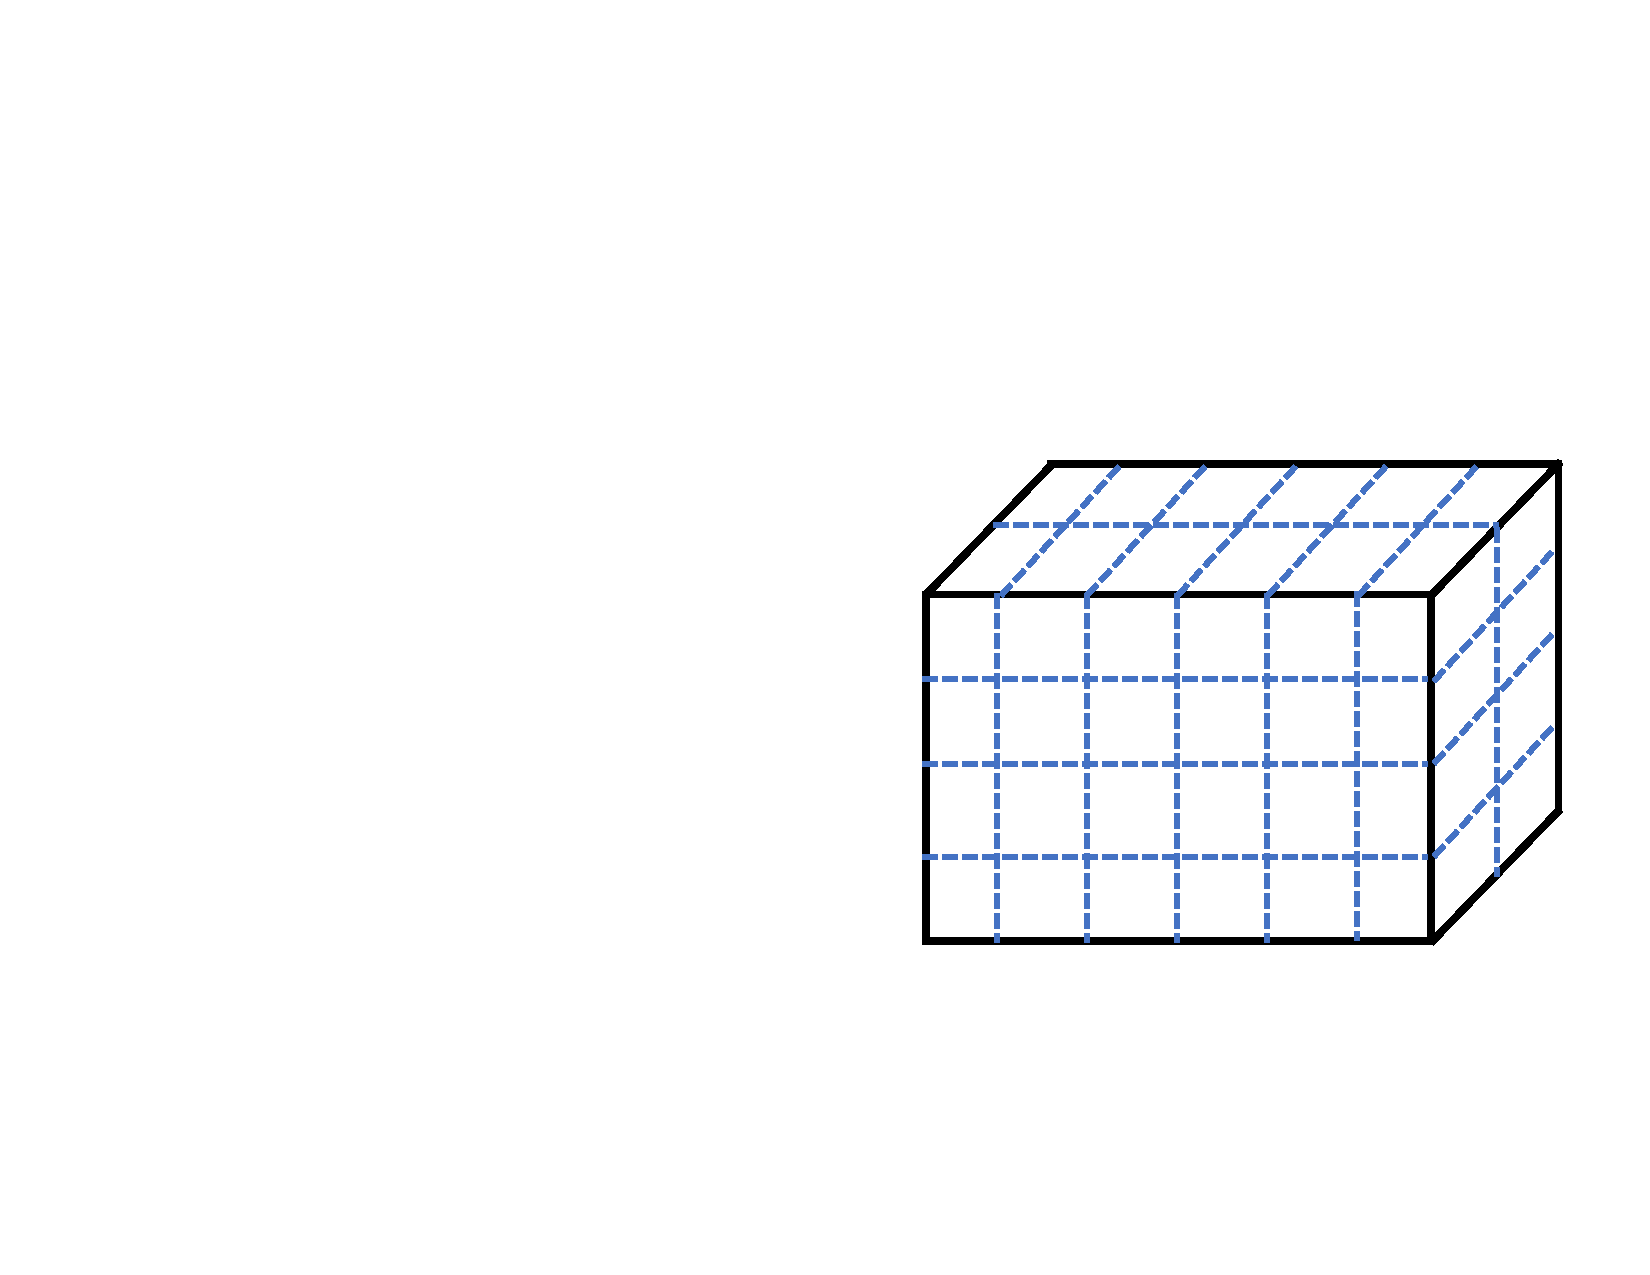
\includegraphics[keepaspectratio=true, width=2.5in]{figs/uniformbox}
   \caption[Uniformly sized box tensor distribution]{Illustration of a uniformly sized box distribution 
 of a three-way tensor to 48 processors}
   \label{fig:uniformbox}
\end{figure}

When using a sampled tensor to estimate the loss function, 
Kolda and Hong~\cite{KH19} scale the contributions of selected
zeros and nonzeros by a factor that amplifies the contribution based on sample
size.  For stratified sampling, they define the estimated loss function 
$\hat F$ (Equation 5.2 of~\cite{KH19}) as 

$$\hat F \equiv \sum_{x_{ijk} \ne 0} \frac{n}{p} f(x_{ijk},m_{ijk}) + 
                \sum_{x_{ijk} = 0} \frac{(N-n)}{q} f(0, m_{ijk}) $$

where the summations are over sampled tensor entries only,
$N$ is the total number indices in the tensor (i.e., the product
of the tensor dimensions), $n$ is the number of tensor nonzeros, $p$ is
the number of nonzeros samples, and $q$ is the number of zero samples.
In distributed memory with local sampling, we locally scale the contributions 
of each index before summing over all processors:
\begin{equation}
\hat F \equiv \sum_{\text{all processors } z} \text{       }
   \sum_{x_{ijk} \ne 0} \frac{n_z}{p_z}  f(x_{ijk},m_{ijk}) +
   \sum_{x_{ijk} = 0} \frac{(N_z-n_z)}{q_z} f(0, m_{ijk})
\label{eq:localloss}
\end{equation}

where the inner summations are over sampled entries, and, on processor $z$, 
$N_z$ is the number of indices in the bounding box 
(i.e., the product of the bounding box dimensions), $n_z$ is the number of 
nonzeros, and $p_z$ and $q_z$ are the numbers of nonzero
and zero samples, respectively.



\section{Algorithm and Parallel Implementation} \label{sec:gcp_alg}

To solve the optimization 
problem in Equation~\ref{eq:gcp}, Kolda and Hong~\cite{KH19} adopt
the Adam optimization algorithm~\cite{KB15} outlined in 
Algorithm~\ref{alg:gcpadam}.
Here, we follow~\cite{KH19} and write the model $\M = [\lambda;\{A_k\}]$,
where $\{ A_k \}$ is the set of factor matrices making up the model.
(In our prior three-way examples, $\{A_k\} = \{A,B,C\}$.)
Algorithm parameters $\alpha$, $\beta_1$, $\beta_2$, $\epsilon$, $\tau$, and
$\nu$ are user-specified parameters controlling the learning rate of 
Adam; we use the default values from TensorToolbox~\cite{TensorToolbox}:
$\alpha=0.001$, $\beta_1=0.9$, $\beta_2=0.999$, $\epsilon=1e-8$, $\tau=1000$, 
and $\nu=0.1$.  Parameter $\ell$ is a lower bound of reasonable solution values
(e.g., $0$ for non-negative tensors).  

\begin{algorithm}
  %\setstretch{1.25}
  \caption{GCP-Adam}
  \label{alg:gcpadam}
  \begin{algorithmic}[1]
    \Function{GCP-Adam}{$\X$, $\M=[\lambda;\{ A_k \}]$, $s$, $\alpha$, $\beta_1$, $\beta_2$, $\epsilon$, $\tau$, $\nu$,  $\ell$}
    \State \label{alg:gcpsetup1} Randomly initialize $\{ A_k \}$
    \State \label{alg:gcpsetup2} $\{ T_k \} \gets 0$; $\{ U_k \} \gets 0$
    \Comment{temporary factor matrices for $\{ A_k \}$}
    \State \label{alg:gcpfsample} $\hat \X \gets $ sparse tensor stratified-sampled from $\X$
    \State \label{alg:gcpfest}$\hat F \gets \textsc{EstObj}(\hat \X, \{ A_k \})$
    \Comment{estimate loss with fixed set of samples}
    \State $t \gets 0$
    \Comment{$t=$ \# of Adam iterations}
    \While{max number of bad epochs not exceded}
    \State Save copies of $\{ A_k \}$, $\{ T_k \}$ and $\{ U_k \}$
    \Comment{save in case of failed epoch}
    \State $\hat F_{\text{old}} \gets \hat F$
    \Comment{save to check for failed epoch}
    \For{$\tau$ iterations}
      \Comment{$\tau = $ \# iterations per epoch}
      \State $\{ G_k \} \gets \textsc{StocGrad}(\X, \{ A_k \}, s)$
      \Comment{$s = $ \# samples per stochastic gradient}
      \For{$k = 1, |\{ A_k \}|$}\tikzmark{AdamTop}
        \State $t \gets t+1$
        \State \label{alg:gcpstart} $T_k \gets \beta_1 T_k + (1-\beta_1) G_k$ 
        \State $U_k \gets \beta_2 U_k + (1-\beta_2) G_k^2$
        \State $\hat T_k \gets T_k / (1-\beta_1^{t})$
        \State $\hat U_k \gets U_k / (1-\beta_2^{t})$
        \State $A_k \gets A_k - \alpha \cdot ( \hat T_k \oslash (\sqrt{\hat U_k}+\epsilon) )$\hspace{3mm}\tikzmark{AdamRight}\tikzmark{AdamBottom}
        \State \label{alg:gcpstop} $A_k \gets \max\{A_k, \ell\}$  
        \Comment{$\ell =$  lower bound}
      \EndFor
    \EndFor
    \State \label{alg:gcbupdatefest} $\hat F \gets \textsc{EstObj}(\hat \X, \{ A_k \})$  \Comment{estimate loss with fixed set of samples}
    \If{$\hat F > \hat F_{\text{old}}$} \Comment{check for failure to decrease loss}
    \State Restore saved copied of $\{ A_k \}$, $\{ T_k \}$, $\{ U_k \}$  \Comment{revert to last epoch's variables}
    \State $\hat F \gets \hat F_{\text{old}}$ \Comment{revert to prior function value}
    \State $t \gets t - \tau$ \Comment{wind back the iteration counter}
    \State $\alpha \gets \alpha \cdot \nu$ \Comment{reduce the step length}
    \EndIf
    \EndWhile
    \State \Return $\Akset$
    \EndFunction
  \end{algorithmic}
  \AddNote{AdamTop}{AdamBottom}{AdamRight}{7cm}{Adam update depends on $\beta_1$, $\beta_2$, $\epsilon$; $\alpha =$ learning rate}
\end{algorithm}


Temporary factor matrices $\{ T_k \}$ and $\{ U_k \}$ are created using the 
same parallel distribution (i.e., the same Tpetra {\tt Maps}) 
as $\{ A_k \}$.  Thus, the randomization and initialization in 
lines~\ref{alg:gcpsetup1}-\ref{alg:gcpsetup2} can be done locally on each
processor's portion of the factor matrices with
no communication.
Likewise, the element-wise factor-matrix operations in 
lines~\ref{alg:gcpstart}-\ref{alg:gcpstop}
can be performed locally; no communication is
needed.

The sparse tensor $\hat \X$ is used to estimate error during GCP-SGD.
It is constructed via stratified sampling using a fixed set of sampled 
indices.
Its creation in line~\ref{alg:gcpfsample} requires communication
to create its maps and import objects relative to $\{ A_k \}$.
The loss function computation in 
line~\ref{alg:gcpfest} requires ``expand'' communication to send the entries of
$\{ A_k \}$ corresponding to indices of $\hat \X$ 
as described Chapter~\ref{sec:mttkrp}; since $\hat \X$ contains zero indices
that were not in $\X$, processors need different factor matrix entries
than they needed for $\X$.  Similarly, expand communication is needed for 
line~\ref{alg:gcbupdatefest} as the entries of $\{ A_k \}$ were modified
by the loop above.

The stochastic gradient computation is by far the most expensive part of 
the GCP-Adam computation.  Algorithm~\ref{alg:sg} provides a high-level
overview of our parallel implementation; mathematical details for stratified
and semi-stratified computation are found in~\cite{KH19}, Algorithms 
4.2 and 4.3, respectively.

In line~\ref{alg:sgsptensor} of Algorithm~\ref{alg:sg}, 
a sampled tensor $\Y$ with $s$ samples is created via stratified or
semi-stratified sampling. The sampling itself is local to each processor, 
but creation of the sampled tensor requires communication to construct its 
maps in each mode.
In line~\ref{alg:sgsystem}, we 
build a {\tt distSystem} class to create the communication
pattern (import objects) between the $\Y$ and $\{ A_k \}$ and expand
values from $\{ A_k \}$ to processors that need them.
Again, $\Y$ may have a different set of zeros from $\X$ and $\hat \X$, so 
different maps and import objects are needed for $\Y$.
In line~\ref{alg:sgdfdm}, the sampled values in $\Y$ are overwritten by
the element-wise partial gradient tensor
such that
$y_{ijk} = \frac{\delta f}{\delta m}(x_{ijk}, m_{ijk})$.
Then MTTKRP operations (line~\ref{alg:sgmttkrp}) 
are used to compute the returned values $\{ G_k \}$.
Only ``fold'' communication of $\{  G_k \}$
is needed during MTTKRP as the values of $\{ A_k \}$
were communicated (expanded) 
during system construction and do not change in the MTTKRP.

Stochastic gradient implementations in TensorToolbox and Genten fuse 
sampling with the partial derivative computation.  They do not form a 
sampled tensor but, rather, sample an index and immediately compute
the element-wise derivative at the index, storing it in $\Y$. They can
do this fusion because they operate in a single memory space and have all 
factor matrix entries available for use.  Since GentenMPI operates in 
distributed memory, it does not have all factor matrix entries associated
with a given sampled index within a processor; those entries must be 
communicated.  We construct the sampled tensor, then, so that the 
communication can be done in one round rather than for each sampled index.



\begin{algorithm}
  \caption{StocGrad}
  \label{alg:sg}
  \begin{algorithmic}[1]
  \Function{StocGrad}{$\X$, $\{ A_k \}$, $s$}
  \State \label{alg:sgsptensor} Sample $s$ indices and construct sparse tensor $\Y$
  \State \label{alg:sgsystem} Build {\tt distSystem} object from $\Y$ and $\{ A_k \}$
  \State \label{alg:sgdfdm} $\Y \gets $ element-wise $\frac{\delta f}{\delta m}$
  \For{$A_m \in \{ A_k \}$}
    \State \label{alg:sgmttkrp} $G_m \gets $ MTTKRP($\Y$, $\{ A_k \} \backslash A_m$)
  \EndFor
  \State return $\{ G_k \}$
  \EndFunction
  \end{algorithmic}
\end{algorithm}


\section{Experimental Results} \label{sec:gcp_exp}

\subsection{Convergence Results}

In this section we present convergence results of GCP-SGD for three different data sets, each using a Poisson loss function and the semi-stratified sampling strategy.
\Cref{fig:chicago_conv,fig:lbnl_conv,fig:amazon_conv} plot the values of the loss function over time.
The first two datasets are small enough to run on a single node, and the first experiment is designed to be compared against an existing result using a MATLAB implementation of the GCP-SGD algorithm \cite{KH19}.
The third data set is too large for GCP-SGD to execute on a single node, and the experiment is performed using 16 nodes.

\begin{figure}
\renewcommand{\datafile}{data/convergence/chicago_conv.dat}
\centering
\begin{tikzpicture}
\begin{axis}[
	ylabel={Error (Poisson loss)}, 
	xlabel={Time (seconds)},
	ymax=2.3e7,
	ymin=2e7,
]
	\addplot table[x=Time, y=Error] {\datafile};    
\end{axis}
\end{tikzpicture}
\caption[GCP-SGD convergence for \emph{Chicago crime data} tensor]{GCP-SGD convergence results for Chicago crime data, using Poisson loss, rank $R=10$, and semi-stratified gradient sampling.  Each of the 92 markers corresponds to an epoch, each epoch corresponds to 1000 iterations, and each iteration used a total of 3152 nonzero samples and 3152 index (zero) samples.  The error is estimated using stratified objective function sampling with 31{,}588 nonzero samples and 31{,}596 zero samples.}
\label{fig:chicago_conv}
\end{figure}

\Cref{fig:chicago_conv} shows the convergence results for GCP-SGD on the \emph{Chicago crime} data set from the FROSTT \cite{FROSTT} collection using Poisson loss.
The Chicago crime data tensor is $6186\times 24\times 77\times 32$ with 5.3 million nonzeros.
This result can be compared against \cite[Figure 5.6]{KH19}, where the same GCP-SGD algorithm is used (with similar parameter settings) in a MATLAB environment.
In both cases, the Poisson loss converges to approximately \texttt{2.05e7}, though the time required is less for the parallel results.
The experiment was performed on a single node of Skybridge, with one MPI process for each of the 16 cores.
The average time per iteration is 1.24 seconds.

\begin{figure}
\renewcommand{\datafile}{data/convergence/lbnl_conv.dat}
\centering
\begin{tikzpicture}
\begin{axis}[
	ylabel={Error (Poisson loss)}, 
	xlabel={Time (seconds)},
]
	\addplot table[x=Time, y=Error] {\datafile};    
\end{axis}
\end{tikzpicture}
\caption[GCP-SGD convergence for \emph{LBNL network} tensor]{GCP-SGD convergence results for LBNL network data, using Poisson loss, rank $R=10$, and semi-stratified gradient sampling.  Each of the 30 markers corresponds to an epoch, each epoch corresponds to 1000 iterations, and each iteration used a total of 439{,}879 nonzero samples and 439{,}881 index (zero) samples.  The error is estimated using stratified objective function sampling with 4{,}398{,}859 nonzero samples and 4{,}398{,}869 zero samples.}
\label{fig:lbnl_conv}
\end{figure}

\Cref{fig:lbnl_conv} shows the convergence results for GCP-SGD on the \emph{LBNL network} data set from the FROSTT \cite{FROSTT} collection using Poisson loss.
The \emph{LBNL network} tensor is $1605 \times 4198 \times 1631 \times 4209 \times 868131 $ with 1.7 million nonzeros.
The experiment was performed on a single node of Skybridge, with one MPI process for each of the 16 cores.
The average time per iteration is 143 seconds.

Compared to the \emph{Chicago crime} data set, the \emph{LBNL network} data set takes over 100 times longer per iteration.
This is because the number of entries in the model is proportional to the sum of the tensor dimensions, and the number of samples used is chosen to be proportional to the number of entries in the model.
That is, the number of samples used for \emph{LBNL network} is about 100 times the number used for \emph{Chicago crime}, which helps to explain the increase in time.

\begin{figure}
\renewcommand{\datafile}{data/convergence/amazon_conv.dat}
\centering
\begin{tikzpicture}
\begin{axis}[
	ylabel={Error (Poisson loss)}, 
	xlabel={Time (seconds)},
]
	\addplot table[x=Time, y=Error] {\datafile};    
\end{axis}
\end{tikzpicture}
\caption[GCP-SGD convergence for \emph{amazon-reviews} tensor]{GCP-SGD convergence results for \emph{amazon-reviews} data, using Poisson loss, rank $R=16$, and semi-stratified gradient sampling.  Each of the 11 markers corresponds to an epoch, each epoch corresponds to 1000 iterations, and each iteration used a total of 4{,}200{,}196 nonzero samples and 4{,}200{,}444 index (zero) samples.  The error is estimated using stratified objective function sampling with 42{,}003{,}186 nonzero samples and 42{,}003{,}214 zero samples.}
\label{fig:amazon_conv}
\end{figure}


\Cref{fig:amazon_conv} shows the convergence results for GCP-SGD on the \emph{amazon-reviews} data set from the FROSTT \cite{FROSTT} collection using Poisson loss.
The experiment was performed on 16 nodes of Skybridge, with one MPI process per core, for a total of 256 MPI processes.
The average time per iteration is 869 seconds.

\subsection{Parallel Distribution for Sampling}

We compare the performance of Algorithm~\ref{alg:gcpadam} using the 
medium-grained distribution and uniform-box distributions described in
Section~\ref{sec:gcp_sample}.  For our experiments, we use the \emph{amazon-reviews}
tensor from the 
FROSTT~\cite{FROSTT} collection.
The Amazon data tensor is $4821207\times 1774269\times 1805187 $ with 1.7 billion nonzeros.
In Figure~\ref{fig:amazon_medgrain_vs_uniformbox}, we show execution times 
for five epochs with 1000 iterations each on
the Skybridge cluster with 128 to 2048 processors.  In all cases, the 
uniform-box distribution resulted in lower execution time and more consistent
scaling performance.  With the uniform-box distribution, less time
was needed for performing MTTKRP and building maps between the sampled tensor and factor matrices.

\begin{figure}
\centering
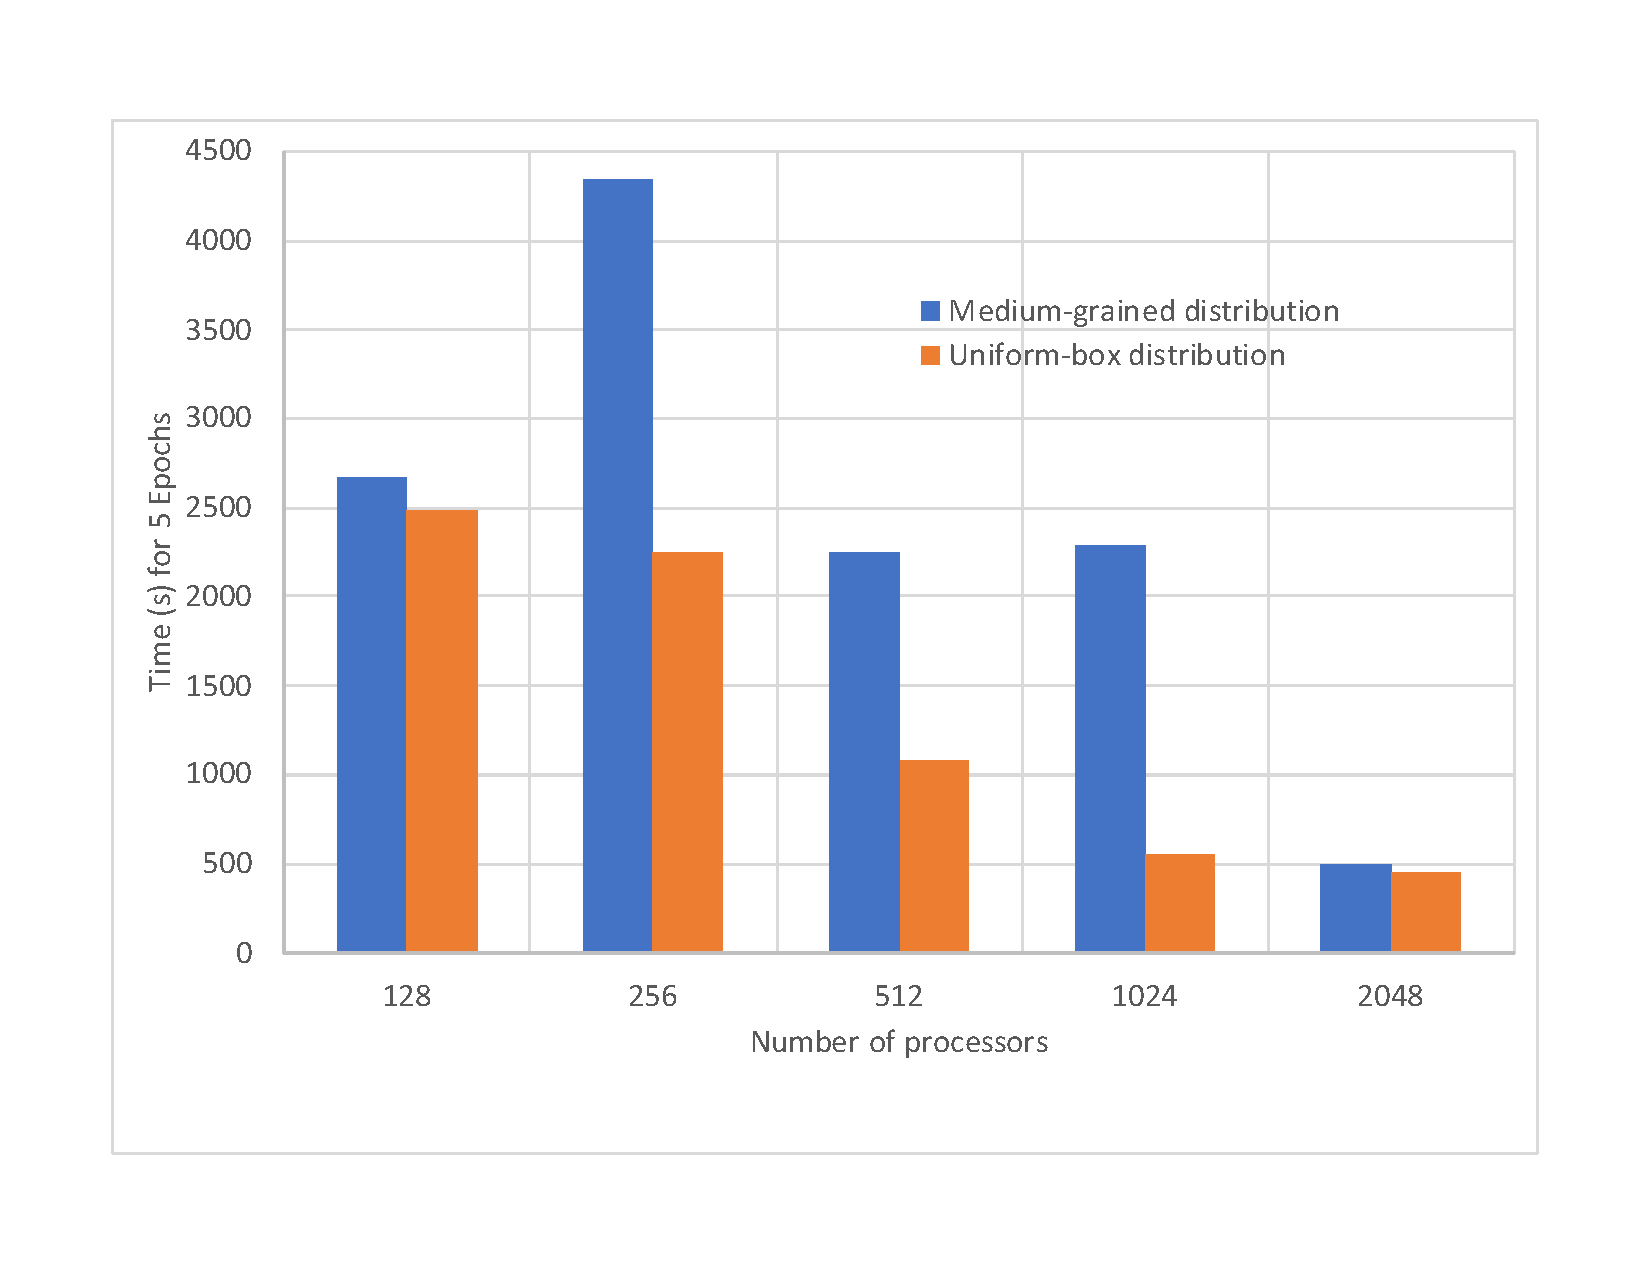
\includegraphics[keepaspectratio=true, width=4.5in]{figs/amazon_medgrain_vs_uniformbox}
\caption[Runtime comparison with medium-grained and uniform-box distributions]{Comparison of runtimes using the \emph{amazon-reviews} tensor using $L^2$ loss, rank $R=16$, and semi-stratified sampling using medium-grained partitioning versus a uniform box distribution.  
Each of the five epochs ran 1000 iterations.  
Each iteration used semi-stratified sampling with approximately 4.2M nonzeros and 4.2M zeros. 
Error estimation used stratified sampling with approximately 42M nonzeros and 42M zeros. 
}
\label{fig:amazon_medgrain_vs_uniformbox}
\end{figure}

Given the benefit of uniform-box distribution, we use it in all subsequent 
parallel experiments.

\subsection{Strong Scaling and Timing Breakdown}

Having confirmed the convergence behavior of GentenMPI, we now consider its parallel performance and strong scaling.
\Cref{fig:lbnl_scaling,fig:random_scaling,fig:amazon_scaling} demonstrate the strong scaling behavior for \emph{LBNL network}, random, and \emph{amazon-reviews} data sets.
All experiments were performed on Skybridge, and all used $L^2$ loss and the semi-stratified sampling strategy.

\begin{figure}
\centering
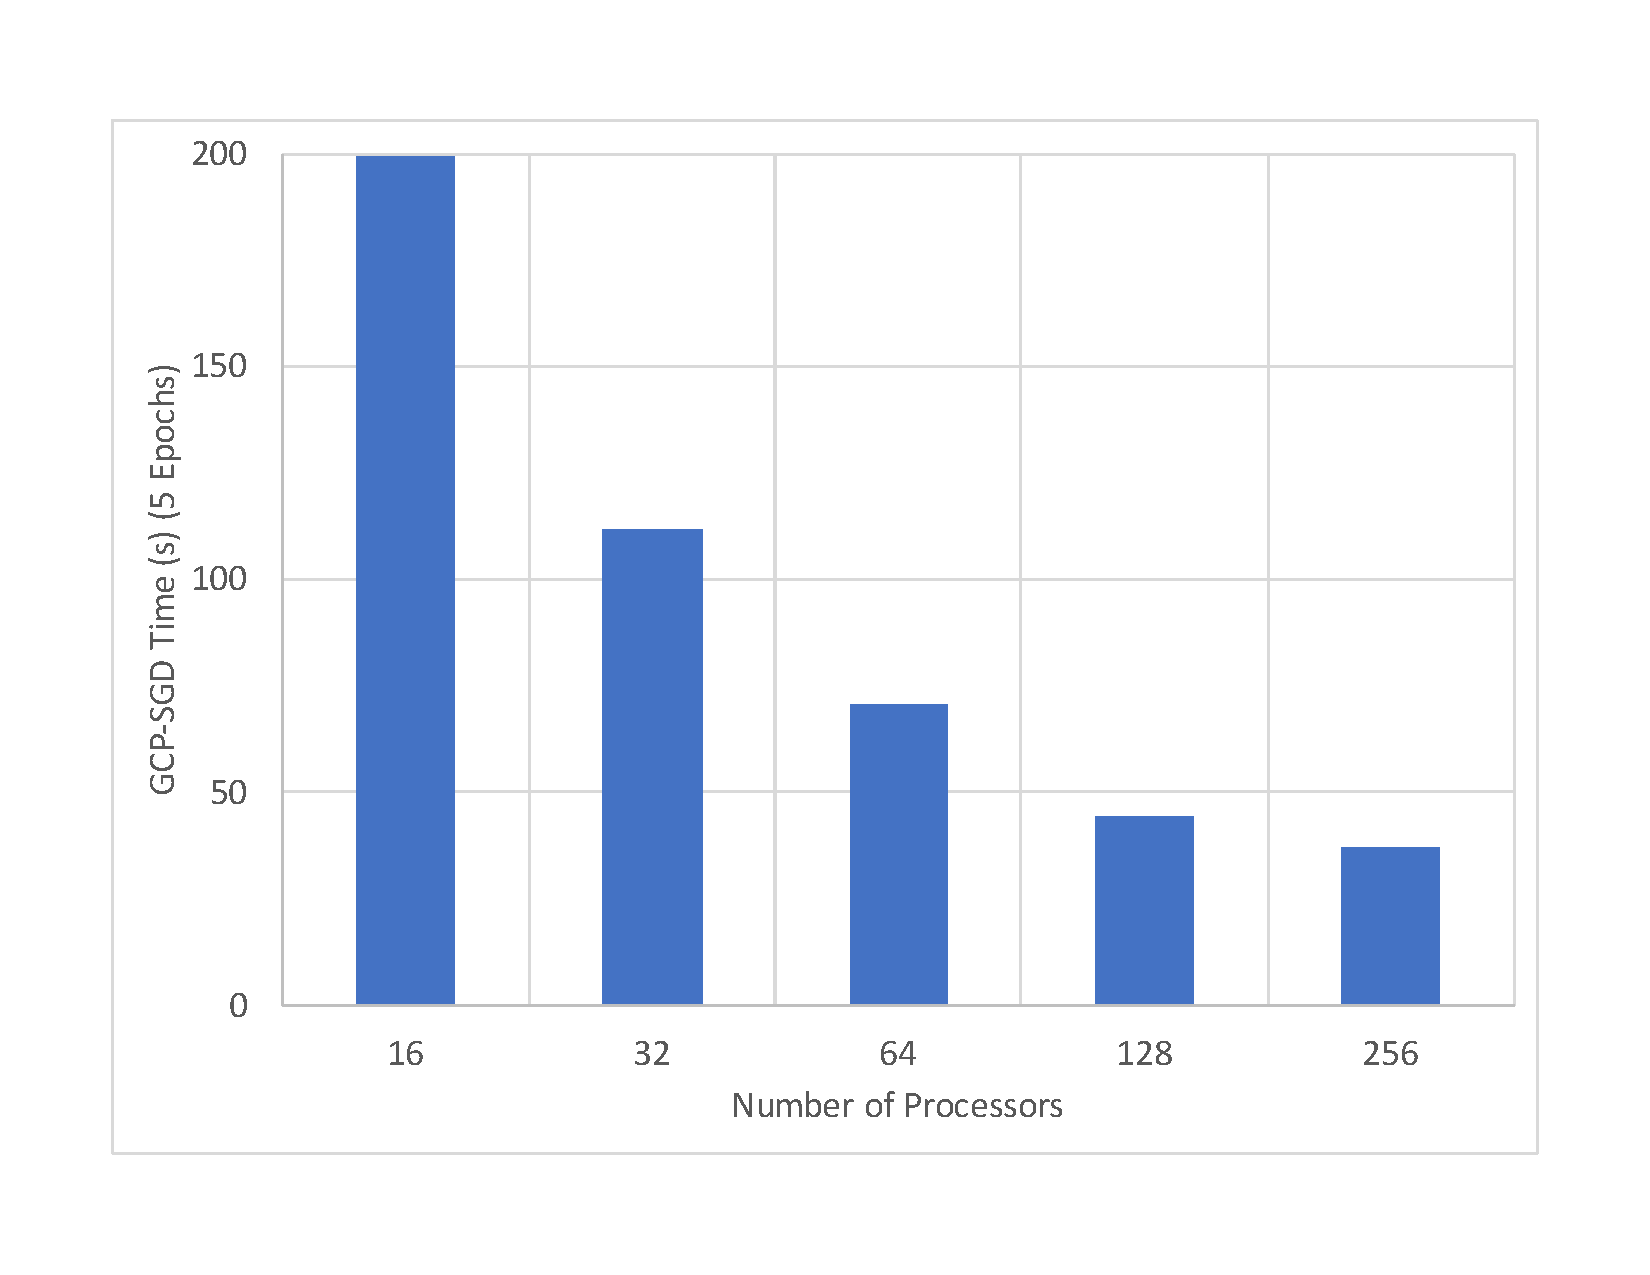
\includegraphics[keepaspectratio=true, width=4.5in]{figs/strongLBNL}
\caption[Strong scaling of GCP-SGD for \emph{LBNL network} tensor]{Strong scaling for \emph{LBNL network} tensor using $L^2$ loss, rank $R=16$, and semi-stratified sampling.  
Each of the five epochs ran 1000 iterations.  
Each iteration used semi-stratified sampling with approximately 10K nonzeros and 10K zeros. 
Error estimation used stratified sampling with approximately 100K nonzeros and 100K zeros. 
}
\label{fig:lbnl_scaling}
\end{figure}

The \emph{LBNL network} data set has order five, with about 1.7 million nonzeros.
For the experimental results in \Cref{fig:lbnl_scaling}, we use approximately 200{,}000 samples to estimate the error and 20{,}000 samples in the stochastic gradient tensor.
On 16 processors (1 node of Skybridge), the time for 5 epochs is 192 seconds.
For comparison, Genten \cite{PK19} takes between 101 and 120 seconds, depending on the MTTKRP implementation used.
The strong scaling is reasonable up to 128 processors, achieving over a $4\times$ speedup, but there is little reduction from 128 to 256 processors.
At 256 processors, the average number of original tensor nonzeros per processor is quite small --- less than 10{,}000 --- and the number of samples per processor is less than 100.

\begin{figure}
\centering
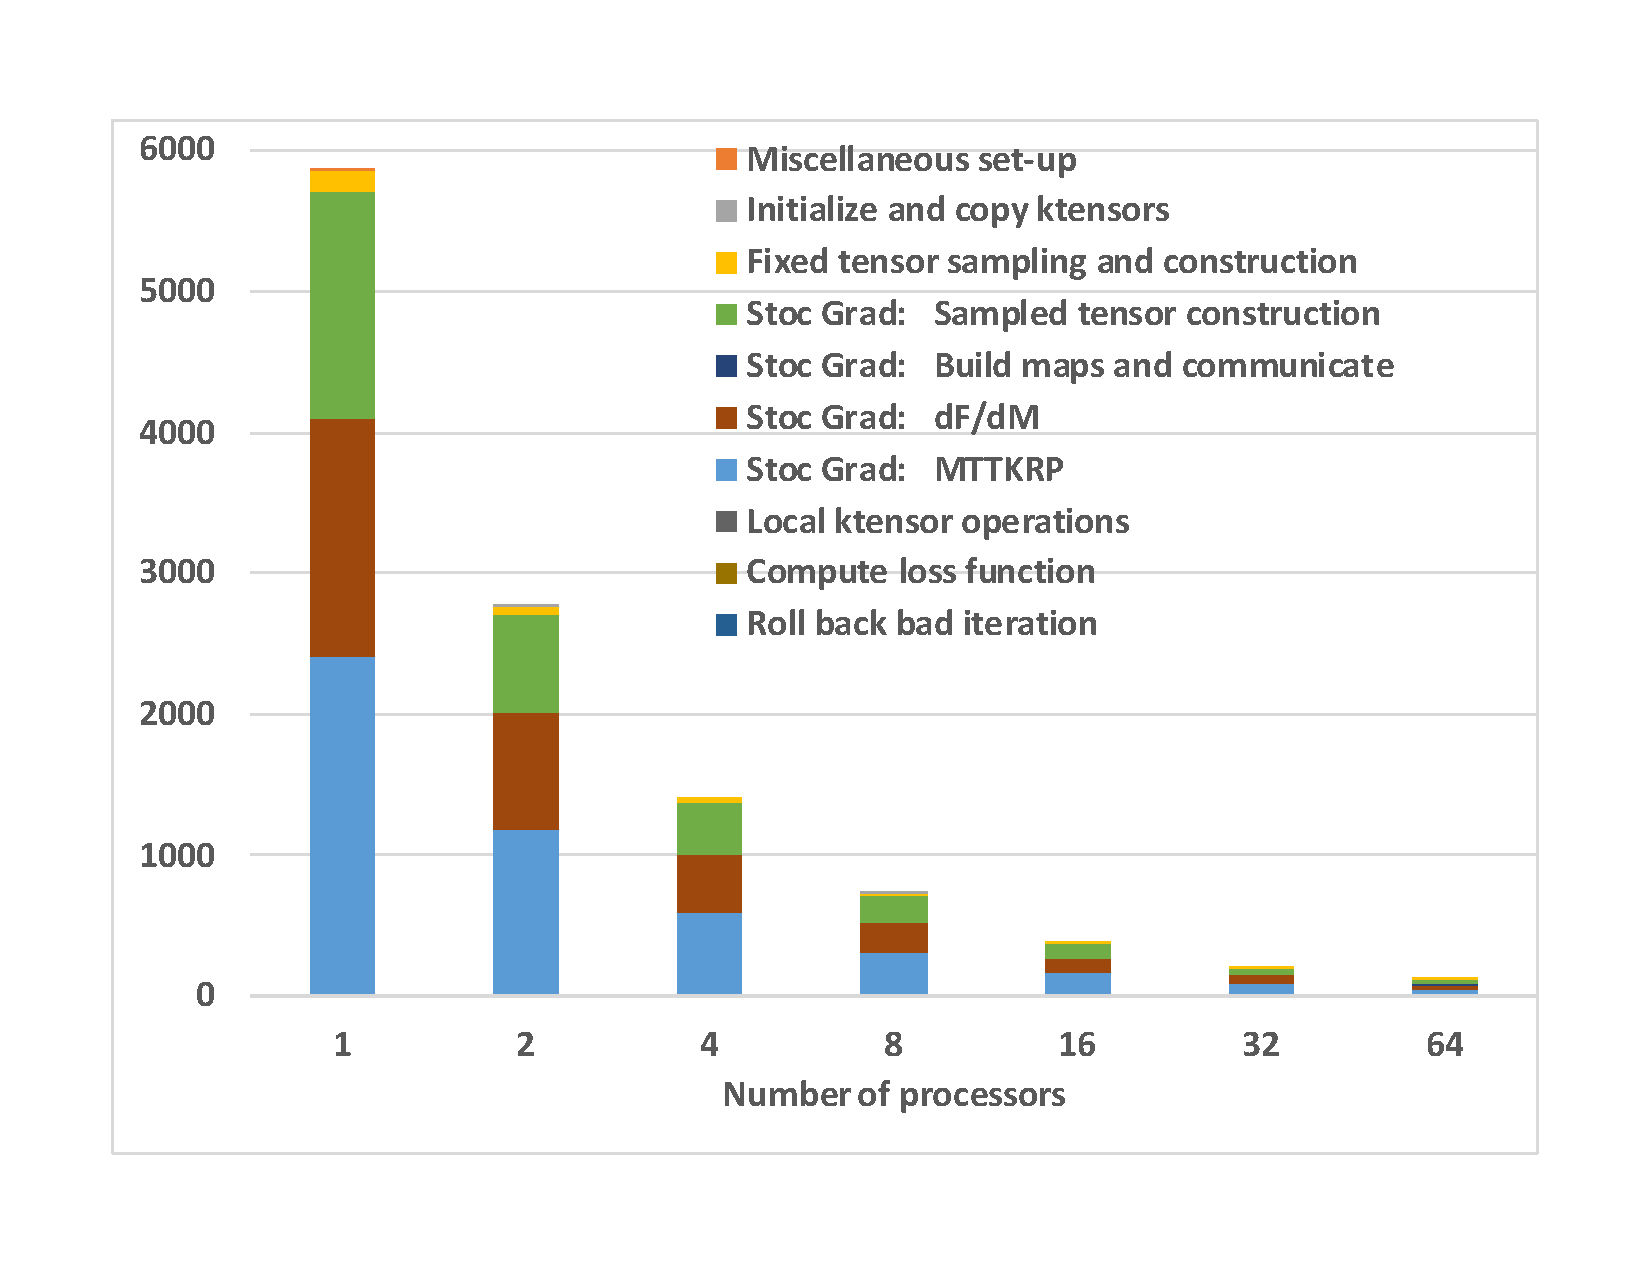
\includegraphics[keepaspectratio=true, width=4.5in]{figs/strongRandomStacked}
\caption[Strong scaling of GCP-SGD for random order-4 tensor]{Strong scaling for random 4D tensor using $L^2$ loss, rank $R=16$, and semi-stratified sampling.  
Each of the five epochs ran 1000 iterations.  
Each iteration used semi-stratified sampling with approximately 768K nonzeros and 768K zeros. 
Error estimation used stratified sampling with approximately 2.6M nonzeros and 2.6M zeros. 
}
\label{fig:random_scaling}
\end{figure}

\Cref{fig:random_scaling} shows experimental results for a random tensor, which allows for perfect load balance of nonzeros, even in the case of uniform boxes.
The random tensor is $1000\times 1000\times 500\times 500$ with 256 million nonzeros.
We use approximately 5 million samples to estimate the error and 1.5 million samples in each stochastic gradient.
Using 16 processors (1 node), GentenMPI took 373 seconds; Genten~\cite{PK19} with 16 threads took between 306 and 1250 seconds, depending on the MTTKRP implementation used.
From one MPI rank to 64 ranks, GentenMPI exhibited a $52.7\times$ speed-up.

From the time breakdown, we see that the dominant kernels in this experiment (using up to 64 processors) are within the stochastic gradient computation: evaluating the partial derivative, constructing the sampled tensor, and performing the MTTKRP.
No communication is needed to evaluate the partial derivative.  Similarly, no communication
is needed to sample the tensor, but a small amount of communication occurs in creating the
Tpetra maps describing the distribution of the sampled tensor 
(see Section~\ref{sec:sptensor}).  
The cost of building maps (the communication pattern) and performing the communication are small in this case, but they grow with the number of processors.

\begin{figure}
\centering
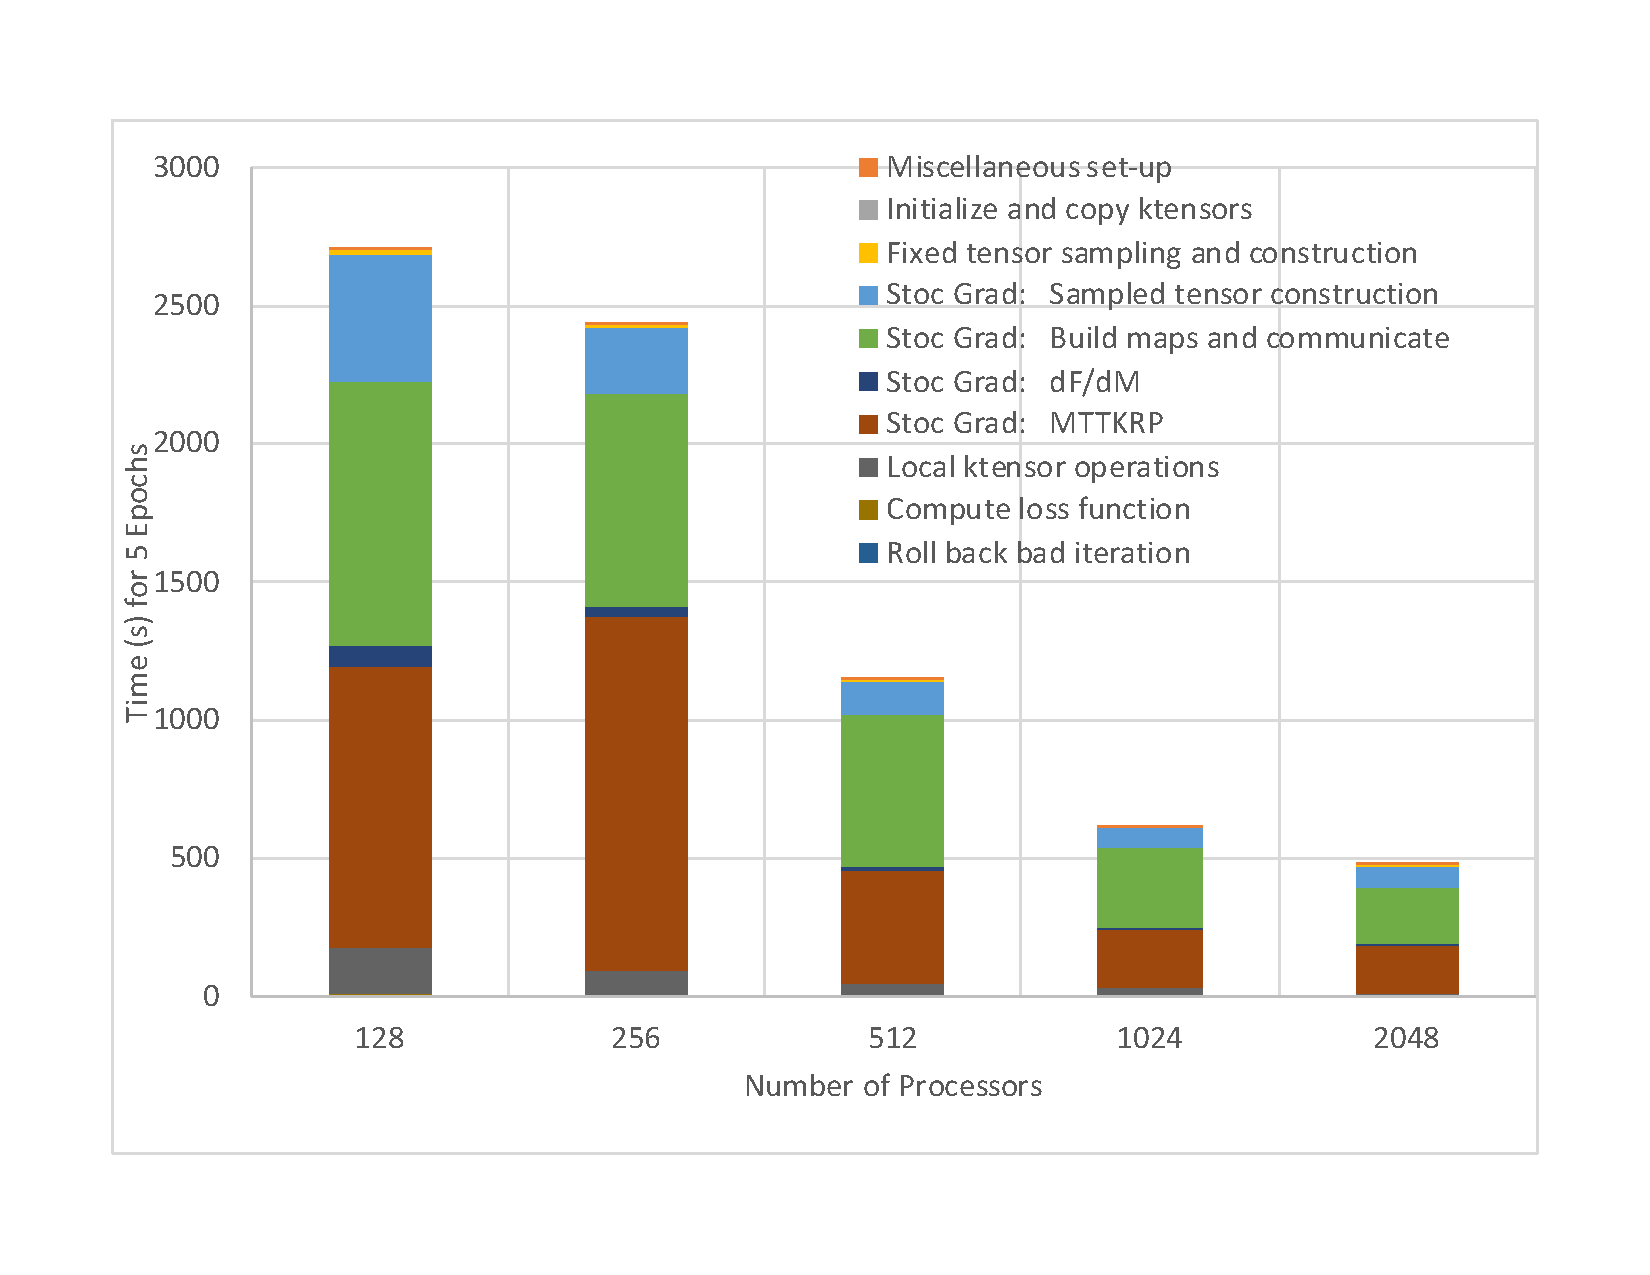
\includegraphics[keepaspectratio=true, width=4.5in]{figs/amazon_stacked}
\caption[Strong scaling of GCP-SGD for \emph{amazon-reviews} tensor]{Strong scaling for \emph{amazon-reviews} tensor using $L^2$ loss, rank $R=16$, and semi-stratified sampling.  
Each of the five epochs ran 1000 iterations.  
Each iteration used semi-stratified sampling with approximately 4.2M nonzeros and 4.2M zeros. 
Error estimation used stratified sampling with approximately 42M nonzeros and 42M zeros. 
}
\label{fig:amazon_scaling}
\end{figure}

\Cref{fig:amazon_scaling} presents results for the \emph{amazon-reviews} tensor, using between 128 and 2048 processors of Skybridge (the tensor is too large to run GCP-SGD on fewer processors).
We use 84 million samples to estimate the error and 8.4 million samples for each stochastic gradient.
Compared to the experiment with the random tensor, we see that communication costs become much more significant in this experiment.
The dominant kernels are again in the stochastic gradient computation, but in this case, the communication costs (building maps and communicating) are significant on 128 processors and become a bottleneck on 2048 processors.
The scaling is nearly perfect between 256 and 1024 processors, but little speedup is obtained in increasing to 2048 processors.

    \chapter{Conclusions and Future Work} \label{sec:conc}

We have described GentenMPI, a toolkit for computing low-rank approximations
of sparse tensors on distributed memory parallel computers.  GentenMPI is built 
on the Trilinos scientific computing toolkit, which provides data structures
and parallel communication classes that can be exploited in tensor 
decomposition.  Using this infrastructure, GentenMPI provides implementations
of the classic CP-ALS low-rank decomposition using alternating least squares
optimization, and the new GCP-SGD method supporting arbitrary loss functions.
We present parallel distribution strategies for sampling tensors in 
distributed memory environments.  And we demonstrate that GentenMPI can achieve 
good parallel scalability, while enabling decomposition of tensors too large
for single-memory computers.

Future work will combine the distributed memory capabilities of GentenMPI with
the multicore- and GPU-capabilities of Genten.  Both Genten and Trilinos rely
on Kokkos for performance-portable multicore and GPU kernels.  On-node
parallelism related to factor matrices and MPI communication packing/unpacking
will be managed by existing Trilinos classes.  On-node parallelism in 
operations such as MTTKRP will exploit methods in Genten.  Some modification
of GentenMPI's tensor storage will be needed to accommodate use of Genten
on the node.  In the end, our
multicore and GPU version of GentenMPI will exploit the fine-grained
parallelism in Trilinos and Genten.



%\begin{table}[ht]
%    \centering
%    \caption[Short Title]{Full caption}
%    \bigskip

%    \begin{tabular}{|l|c|l|c|}
%    \end{tabular}
%    \label{tab:1}
%\end{table}

%\begin{figure}[ht]
%    \centering
%    \subfigure[Short title]{
%	\label{fig:sub:1}
%	\includegraphics[keepaspectratio=true, width= in]{filename}
%    }
%    \subfigure[Short title]{
%	\label{fig:sub:2}
%	\includegraphics[keepaspectratio=true, width= in]{filename}
%    }
%    \caption{Full caption.}
%    \label{fig:1}
%\end{figure}



    % ---------------------------------------------------------------------- %
    % References
    %
    \clearpage
    % If hyperref is included, then \phantomsection is already defined.
    % If not, we need to define it.
    \providecommand*{\phantomsection}{}
    \phantomsection
    \addcontentsline{toc}{chapter}{References}
    \bibliographystyle{plain}
    \bibliography{refs}


    % ---------------------------------------------------------------------- %
    %
%    \appendix
%    \chapter{}

    % \printindex

    \begin{SANDdistribution}[NM]% or [CA]
	% \SANDdistCRADA	% If this report is about CRADA work
	% \SANDdistPatent	% If this report has a Patent Caution or Patent Interest
	% \SANDdistLDRD	% If this report is about LDRD work

	% External Address Format: {num copies}{Address}
	\SANDdistExternal{}{}
	\bigskip

	% The following MUST BE between the external and internal distributions!
	% \SANDdistClassified % If this report is classified

	% Internal Address Format: {num copies}{Mail stop}{Name}{Org}
	\SANDdistInternal{}{}{}{}

	% Mail Channel Address Format: {num copies}{Mail Channel}{Name}{Org}
	\SANDdistInternalM{}{}{}{}
    \end{SANDdistribution}


    % The second printing
    %\begin{SANDreDistribution}
    %    \SANDdistExternal{}{}
    %    \bigskip
    %    \SANDdistInternal{}{}{}{}
    %    \SANDdistInternalM{}{}{}{}
    %\end{SANDreDistribution}

\end{document}
